\documentclass[11pt,twoside]{book}

% this requres the installation of texlive-pstricks, as that is needed
% by the vaucanson-g.sty and VCColor-names.def files

\usepackage{palatino}
\usepackage{url}
\usepackage{epsfig}
\usepackage{listings}
\usepackage[table]{xcolor}
\usepackage{wrapfig}

\setlength{\headheight}{0pt}
%\setlength{\footheight}{0pt}
\setlength{\topmargin}{-.5in}
\setlength{\oddsidemargin}{-0.25in}
\setlength{\evensidemargin}{-0.25in}
\setlength{\textwidth}{7truein}
\setlength{\textheight}{9.0truein}
\setlength{\parskip}{6pt}

\newcommand{\und}[1]{\underline{\smash{#1}}}
\newcommand{\leftshift}{<<}

\newenvironment{itemlist}{
\begin{itemize}
\setlength{\itemsep}{0pt}
\setlength{\parskip}{0pt}}
{\end{itemize}}

\newenvironment{numlist}{
\begin{enumerate}
\setlength{\itemsep}{0pt}
\setlength{\parskip}{0pt}}
{\end{enumerate}}

\raggedbottom

\lstset{frameround=fttt,captionpos=b}

\begin{document}

\title {Program and Data Representation}
\author {by Aaron Bloomfield}
\maketitle

\cleardoublepage
\pagenumbering{roman}
\addcontentsline{toc}{part}{Table of Contents}
\tableofcontents

\cleardoublepage
\addcontentsline{toc}{part}{List of Figures}
\listoffigures

\cleardoublepage
\addcontentsline{toc}{part}{List of Tables}
\listoftables

\cleardoublepage
\addcontentsline{toc}{part}{List of Listings}
\lstlistoflistings

\cleardoublepage
\pagenumbering{arabic}

\chapter{Introduction}

\section{Purpose}

\section{How to use this book}

\section{History}



\part{C++}

\chapter{Introduction}

\section{Hello world}

\section{Data types}

\section{Control structures}

\section{Classes and objects}

\section{Header files}



\chapter{Pointers, References, and Memory Management}

\section{Pointers}

\section{Dynamic memory allocation}

\section{References}


\chapter{Arrays}


\chapter{Standard Template Library}

\section{Introduction}

\section{\tt vector}

\section{\tt linked\_list}

\section{\tt string}

\section{\tt \ldots}


\chapter{Advanced C++ Concepts and C++11}

\section{Inheritance}

\section{Dynamic dispatch}

\section{Templates}


\part{Data Structures}

\chapter{Big-Oh Comparisons}

\section{Introduction}

\section{Big-Oh versus Big-Theta versus Big-Omega}

\section{Formal proofs}


\chapter{Lists}

\section{Linked lists}

\section{Stacks}

\section{Queues}


\chapter{Trees}

\section{Binary trees}

\section{Binary search trees}

\section{AVL trees}

\section{Red-black trees}

\section{Splay trees}

\section{Other tree applications}



\chapter{Hashes}

\section{Hash functions}

\section{The hash table}

\section{Collision resolution}

\section{Analysis}


\chapter{Heaps}

\section{Structure property}

\section{Ordering property}

\section{Array storage}

\section{Huffman coding}


\chapter{Graphs}

\section{Introduction}

\section{Representation}

\section{Topological sort}

\section{Traveling salesperson}

\section{Shortest path}

\section{Minimum spanning tree}



\part{Data Representation}

\chapter{Integers}

\section{Sign-and-magnitude}

\section{One's complement}

\section{Two's complement}

\section{BigInteger representation}


\chapter{Floating-point Numbers}

\section{Older representations}

\section{IEEE 754 floating point standard}



\chapter{Strings}

\section{ASCII versus UNICODE}

\section{String representation}


\chapter{Memory}

\section{\ldots}

\part{Assembly and Machine Language}

\chapter{IBCM: The Itty Bitty Computing Machine}
\lstset{frameround=fttt,captionpos=b}

\begin{quotation} {\em 
\noindent
The child receives data through the sense organs; the child also has
some inborn processing capacities~-- otherwise it would not be able
to learn~-- but in addition, some ``information'' or ``programs'' are
built-in at birth
%(for example, the child does not have to learn how to suck, for this
%is an innate reflex); 
\ldots
there is a working memory
%, in which the child keeps those items of knowledge that are being
%used at a particular moment;
\ldots
and there is a permanent memory
%, which is, in Locke's terms, largely a ``blank tablet'' at birth, but
%which has a storage capacity that makes a hard disk pale into
%insignificance.  The child gradually builds up a symbolic
%representation of the world around it, 
\ldots
so there must be some inner ``language'' or medium of representation
%; even a newborn baby is starting to see and taste and smell and hear
%and touch, and to remember the more striking of its experiences, so
%the internal medium by which it represents and stores these
%impressions cannot be the native language (of which it is still
%ignorant. 
\ldots 
Jerry Fodor
%[in The Language of Thought]
\ldots
has discussed this inbuilt ``language of thought,'' which is similar
conceptually to the ``machine language'' that is built into the
personal computer.
%and about which most users remain completely ignorant).
}

-- John Cleverly, in ``Visions of childhood: Influential models from
Locke to Spock'' \cite{cleverley1986visions}
\end{quotation}


\section{Introduction}

{\bf Machine language}, or {\bf machine code}, is the set of
instructions that a computer's central processing unit (CPU)
understands.  It is the binary 0's and 1's that form instructions for
the CPU to execute.  When we compile a program, that program is
eventually converted to binary machine code, which we can then run.
Each different CPU has a different machine language that it
understands, although CPU families tend to understand a very similar
language.

Programming in machine language requires one to write the code in
hexadecimal notation, manually encoding the instructions one at a
time.  For this reason, machine language can often be difficult to
program in.  This is especially true with the complexities of modern
instruction sets on processor families such as the x86 and MIPS.

One will often write a program in {\bf assembly language}, which is a
(somewhat) higher-level manner to create a program.  In assembly
language, one can specify to add two values together through a command
such as {\tt sub esp, 24}, and need not write it in the hexadecimal
notation of 0x83ec20.
% to get that value, compile test_abs_c.c via: 'g++ -m32 -o test_abs_c
% test_abs_c.c', load it into gdb, and run 'disassemble /r main'.
% It's the 4th line (or so) of the main function.
An {\bf assembler} is a program that converts assembly language into
machine language.  In fact, compilers typically produce assembly
language, and then call the assembler to produce the machine code.

Learning how machine language works allows us to truly understand how
a machine operates at a very low level.

In this chapter we introduce a simplified machine language called the
Itty Bitty Computing Machine, or IBCM.  This machine language is
designed to be simple enough that it can be learned in a reasonable
amount of time, but complex enough that one can use it to write a wide
range of programs.  It is intended to teach many of the important
concepts of a modern machine language without having to deal with the
complexities of~-- and time required to learn~-- modern CPU machine
languages.


\section{Memory Hierarchy}

Typically, computer programs do not differentiate between the various
levels of memory.  Programs tend to view memory as a monolithic whole,
and allocate memory as needed.  In fact, there are many different
levels of memory.  Fast memory~-- formally called {\em static
  random-access memory} or SRAM~-- is expensive to make, and computers
would be quite expensive if all memory were fast memory.  In fact,
some super computers did just this~-- the Cray Y-MP, a super computer
from the late 1980's, used only SRAM, and it cost approximately 10
million dollars.
% http://en.wikipedia.org/wiki/Cray_Y-MP
% cost: http://www.geek.com/articles/news/cray-for-sale-on-ebay-2000097/

Instead, most computers use primarily {dynamic random-access memory},
or DRAM, as the primary component of main memory, and use a smaller
amount of SRAM to speed up computations.  SRAM is used in the {\em
  cache}, although we will not go into detail about caches here.

\begin{wrapfigure}{r}{0.55\textwidth}
\begin{center}
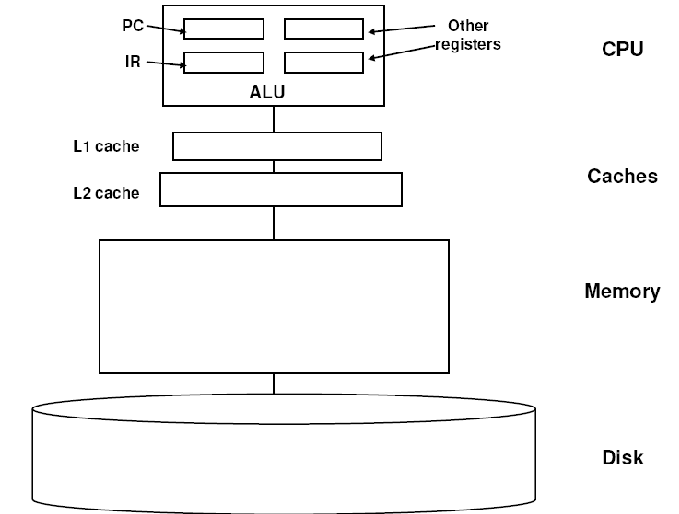
\includegraphics[width=4in]{ibcm/memory-hierarchy.png}
\end{center}
\caption{Memory Hierarchy}
\label{memory-hierarchy}
\vspace{-0.6in}
\end{wrapfigure}

The four primary levels of memory are listed below.  Cost decreases
and storage capacity increases as one moves down the list.

\begin{itemlist}
\item CPU registers
\item Static random-access memory (SRAM) in various levels of cache
  (L1 cache, L2 cache, etc.)
\item Dynamic random-access memory (DRAM) used in main memory
\item Hard drive storage, either on a traditional hard disk with
  rotating platters, or on solid state hardware.
\end{itemlist}

This chapter will largely ignore storing data in cache or on the hard
drive, as that is typically managed by the operating system.  Instead,
we will primarily focus on the values kept in the registers in a CPU,
and in main memory.

Main memory is relatively slow, compared with the speed of a CPU.  In
addition, many CPUs can only allow one memory access per instruction.
Thus, the other values must be kept in a location that is not main memory:
the CPU's registers.  A register is a small area of memory in the CPU
where intermediate computation values can be stored.  A modern CPU
will have registers that each are 32 or 64 bits in size, and may have
12-32 of these registers.

Thus, there are instructions~-- in both machine language and assembly
language~-- that move data between the CPU's registers and main memory.
We will see these instructions shortly.



\section{IBCM Principles of Operation}

\subsection{Machine Description}

The Itty Bitty Computing Machine (IBCM) is a very simple computer.  In
fact, it's so simple that no one in their right mind would build it
using today's technology. Nevertheless~-- except for limits on problem
size~-- any computation that can be performed on the most modern,
sophisticated computer can also be performed on the IBCM.  Its main
virtues are that it can be taught quickly and provides context for
talking about more recent architectures.

The IBCM contains a single register, called the accumulator.  Most
early computers had just an accumulator, and many current
micro-controllers are still accumulator machines.  IBCM's accumulator
can hold a 16-bit 2's complement integer.  In addition, the IBCM has
two other registers: the instruction register (IR), which contains the
current instruction being executed, and the program counter (PC),
which contains the address of the next instruction to be executed.
However, we will not directly use those two registers.

The IBCM has 4,096 addressable memory locations and each of these
locations holds 2 bytes (16 bits).  Thus, the IBCM technically has
8,192 bytes (8 Kb) of memory.

The IBCM handles input by reading in single values (either a
hexadecimal value or an ASCII character) into the accumulator.
Similarly, output is handled by writing the value in the accumulator
as either a hexadecimal value or an ASCII character.

\subsection{Instructions}

The IBCM equivalent of ``statements'' in a higher level language are
very simple instructions.  Each instruction is encoded in a 16-bit
word in one of the formats shown in
Figure~\ref{IBCMInstructionFormat}.  Shaded areas in the figure
represent portions of the instruction word whose value does not
matter. For example, a word whose leftmost four bits are zero is an
instruction to halt the computer.


\begin{figure}[h!]
\centering
%\begin{tabular}{cccccccccc}
\begin{tabular}{cccccp{1mm}p{1mm}ccr|lc}

bit: & 15 & 14 & 13 & 12 & 11 & 10 & \ldots &  & \multicolumn{1}{r}{0} & \\
\cline{2-10}

& \multicolumn{1}{|c}{0} & 0 & 0 & \multicolumn{1}{c|}{0} &
\cellcolor[gray]{0.8} & \cellcolor[gray]{0.8} &
(unused)\hspace{0.25in}\cellcolor[gray]{0.8}&\cellcolor[gray]{0.8} &
\cellcolor[gray]{0.8} 
& halt & \multicolumn{1}{c}{\begin{tabular}{c}\\\\\end{tabular}} \\
\cline{2-10}

& \multicolumn{1}{|c}{0} & 0 & 0 & \multicolumn{1}{c|}{1} &
\multicolumn{2}{p{2mm}|}{\begin{tabular}{l}\hspace{-0.075in}I/O\\\hspace{-0.025in}op\\\end{tabular}}
& (unused) \cellcolor[gray]{0.8}& \cellcolor[gray]{0.8} &
\cellcolor[gray]{0.8} & I/O & \\ \cline{2-10}

& \multicolumn{1}{|c}{0} & 0 & 1 & \multicolumn{1}{c|}{0} &
\multicolumn{2}{p{2mm}|}{\begin{tabular}{l}\hspace{-0.09in}shift\\\hspace{-0.025in}op\\\end{tabular}}
& \hspace{0.25in}(unused)\hspace{0.25in} \cellcolor[gray]{0.8}&
\multicolumn{2}{|c|}{count} & shifts & \\ \cline{2-10}

& \multicolumn{4}{|c|}{opcode} & \begin{tabular}{cc}\\\\\end{tabular} &
& address & & & others & \\ \cline{2-10}

\end{tabular}
\caption{IBCM instruction format}
\label{IBCMInstructionFormat}
\end{figure}

A note on using hexadecimal notation: IBCM is a binary computer.
Internally all operations are performed on 16-bit binary values.
However, because it's so tedious and error-prone for humans to write
or read 16-bit quantities, all of IBCM's input/output is done either
as ASCII characters or 4-digit hexadecimal numbers.  Remember that
these are just external shorthands for the internal 16-bit values!

Also, hexadecimal values are often prefixed by a '0x', such as
'0x1234'.

\subsubsection{Halt}
Any instruction where the opcode is zero (i.e., the first 4 bits are
all zero) will halt the IBCM.  It does not matter what the remaining
12 bits are.  Not much else to say on this one.

\subsubsection{Input and Output}

The input and output (or 'I/O') instructions move data between the
accumulator and the computer 'devices'~-- the keyboard and screen.
Data can be moved either as hexadecimal numbers or as an ASCII
character; in the later case, only the bottom (least significant) 8
bits of the accumulator are involved. The next two bits after the
opcode specify if the instruction is an input or output, and if it
will use hexadecimal values or ASCII characters.  The four
possibilities (in/out, hex/ASCII) that are specified by the bits 11 and
10 of the instruction word as shown in
Table~\ref{IBCM-io-instruction-values.tbl}.  Being as there are only
four possibilities, the full hexadecimal encoding of each of the four
I/O instructions is also listed.

\begin{table}[h]
\centering
\begin{tabular}{ccclcl}
\und{bit 11} & \und{bit 10} & & \und{operation} & & \und{hex value} \\
0 & 0 & & read a hexadecimal word (four digits) into the accumulator &
& 0x1000 \\
0 & 1 & & read an ASCII character into the accumulator bits 8-15 & &
0x1400 \\
1 & 0 & & write a hexadecimal word (four digits) from the accumulator
& & 0x1800 \\
1 & 1 & & write an ASCII character from the accumulator bits 8-15 & &
0x1c00 \\
\end{tabular}
\caption{IBCM input/output bit values}
\label{IBCM-io-instruction-values.tbl}
\end{table}

\subsubsection{Shifts and Rotates}

Shifting and rotating are common operations in computers. Shifting
means moving data to the right or left; rotating is much the same
thing except that bits that ``fall off'' one end are reinserted at the
other end.  

The examples below assume that the value being rotated is one byte (8
bits) in length. In reality, the IBCM performs shifts and rotates on
the 16 bit value in the accumulator.  We choose to describe these
operations with 8 bit quantities to make the explanation easier to
understand.

Diagrammatically, a ``right shift'' of ``$n$ positions'' looks like
Figure~\ref{ibcm-shift-1} when $n = 3$:

\begin{figure}[h]
\centering
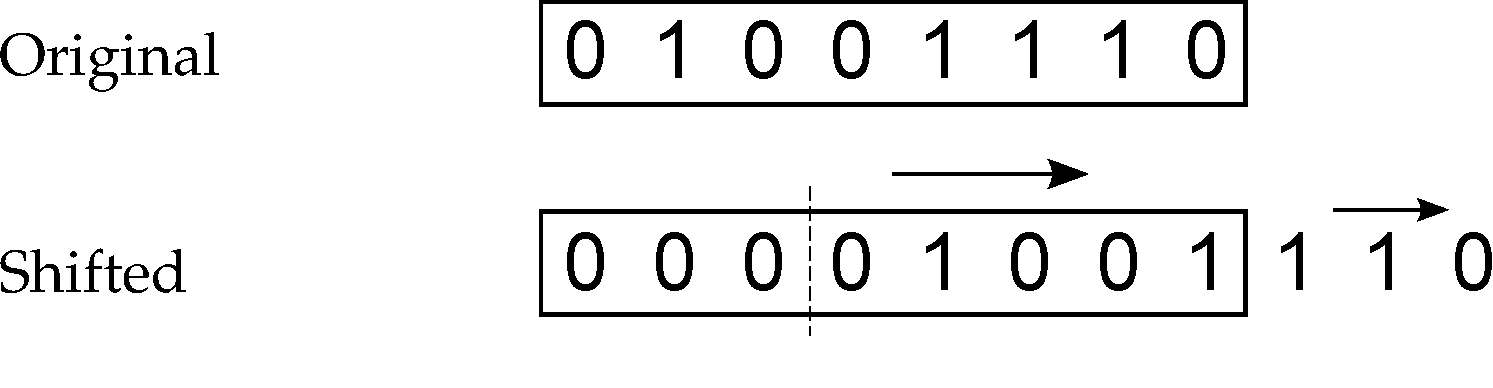
\includegraphics[width=4in]{ibcm/ibcm-shift-1.pdf}
\caption{A right shift of 3}
\label{ibcm-shift-1}
\end{figure}

Each bit is moved $n$ positions to the right (three in this case).
Alternatively, it is moved one bit to the right $n$ times. This causes
the original $n$ right-most bits to fall off the right end and $n$ new
(zero) bits to be inserted at the left end. A ``left shift'' is much
the same, except that bits move to the left, as shown in
Figure~\ref{ibcm-shift-2}.

\begin{figure}[h]
\centering
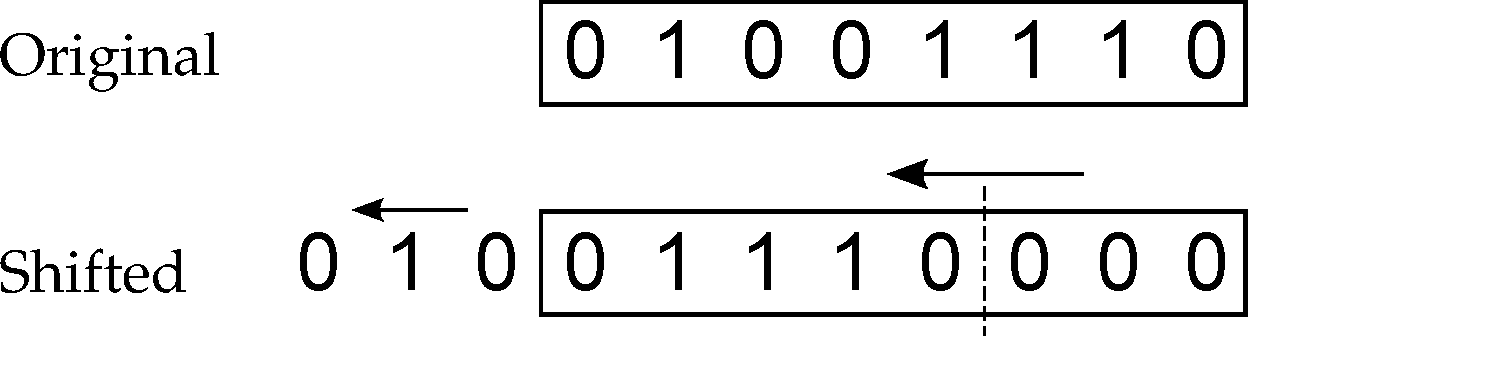
\includegraphics[width=4in]{ibcm/ibcm-shift-2.pdf}
\caption{A left shift of 3}
\label{ibcm-shift-2}
\end{figure}

As noted previously, rotates are like shifts except that the bits that
fall off one end but are reinserted at the other end.
Figure~\ref{ibcm-shift-3} is a left rotation; right rotates are left
to your imagination.

\begin{figure}[h]
\centering
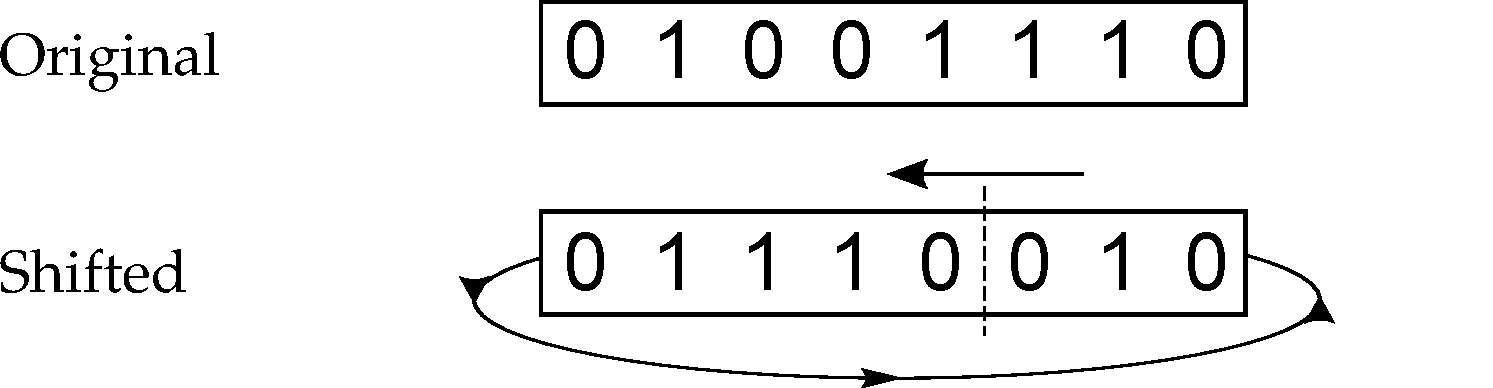
\includegraphics[width=4in]{ibcm/ibcm-shift-3.pdf}
\caption{A left rotation of 3}
\label{ibcm-shift-3}
\end{figure}

Note that the shift instructions uses bits 11-10 to specify the shift
operation.  The first bit specifies if it is a shift (0) or rotate
(1), and the second bit specifies if it is moving left (0) or right
(1).  This is shown in Table~\ref{IBCM-shift-instruction-values.tbl}.

\begin{table}[h]
\centering
\begin{tabular}{cccl}
\und{bit 11} & \und{bit 10} & & \und{operation} \\
0 & 0 & & shift left \\
0 & 1 & & shift right \\
1 & 0 & & rotate left \\
1 & 1 & & rotate right \\
\end{tabular}
\caption{IBCM shift/rotate bit values}
\label{IBCM-shift-instruction-values.tbl}
\end{table}

In addition, bits 3-0 of the shift instructions specify the ``shift
count''~-- that is, the number of bits positions that the data is to
be shifted (or rotated).

A left rotate of 3, which is what is shown in
Figure~\ref{ibcm-shift-3}, would have the opcode set to 2 (binary
0010), the shift/rotate bit set to 1, the left/right bit set to 0, and
the shift count set to 3.  The encoded instruction, in binary, is
shown in Figure~\ref{IBCM-right-rotate-of-3}.  Note that the
grayed-out part of the table are the bits whose value does not matter;
we set them to 0.

\begin{figure}[h!]
\centering
\begin{tabular}{|c|c|c|c|c|c} \cline{1-5}
0 0 1 0 & 1    &  0   &\cellcolor[gray]{0.8} 0 0 0 0 0 0 & 0 0 1 1 & =
0x2803 \\ \cline{1-5}
opcode  & rot. & left &\cellcolor[gray]{0.8} unused & shift \\
        & bit  & bit  &\cellcolor[gray]{0.8} bits   & count \\ \cline{1-5}
\end{tabular}
\caption{IBCM instruction for a right rotate of 3}
\label{IBCM-right-rotate-of-3} 
\end{figure}

As shown in the table, the hexadecimal encoding of the instruction is 0x2803.

\subsubsection{Other Instructions}

All other bit combinations in the left-most four bits either specify
an arithmetic instruction or a control instruction~-- similar to
assignment statements and {\tt goto}s in a high level language. The first four
bits are called the ``op'' field of the instruction; the value of this
field is often called the ``opcode''. The ``address'' portion of the
instruction generally specifies an address in memory where an operand
(variable) will be found.

There are 13 IBCM operations of this form~-- eight that manipulate
data and five that perform control. The data manipulation operations
all involve the ``accumulator'' and typically data from a memory
location is specified by the address portion of the instruction (the
{\tt not} and {\tt nop} instructions are the only two different ones).
The result of data manipulation operations is recorded in the
accumulator.  Thus, the ``add'' instruction forms the arithmetic sum
of the present contents of the accumulator with the contents of the
memory location specified by ``address'' and puts the result back into
the accumulator. Thus, it is similar to the primitive assignment
statement ``{\tt accumulator = accumulator + memory[address]}''.

The control instructions determine the next instruction to be
executed. The ``jump'' instruction, for example, causes the next
instruction executed to be the one at the location contained in its
address field. If you think of the address of a memory cell like a
label in a high level language, then jump is just ``{\tt goto
  address}''.

Two of the control instructions are conditional; they either cause a
change in the control flow or not, depending on the value of the
accumulator. The simplest of the control instruction is {\tt nop}; it
does nothing.

Table~\ref{IBCMopcodes.tbl} describes the function of each of these 13
IBCM instructions; both English and programming language-like
explanations are given for each instruction. In the latter, ``a'' is
the accumulator, ``addr'' is the value of the address portion of the
instruction, and ``mem[]'' is memory.

\begin{table}[h]
\centering
\begin{tabular}{llll}
\und{op} & \und{name} & \und{HLL-like meaning} & \und{English explanation} \\
3$_{16}$ & load  & a := mem[addr]       & load accumulator from memory \\
4$_{16}$ & store & mem[addr] := a       & store accumulator into memory \\
5$_{16}$ & add   & a := a + mem[addr]   & add memory to accumulator \\
6$_{16}$ & sub   & a := a - mem[addr]   & subtract memory from accumulator \\
7$_{16}$ & and   & a := a \& mem[addr]  & logical 'and' memory into accumulator \\
8$_{16}$ & or    & a := a $|$ mem[addr] & logical 'or' memory into accumulator \\
9$_{16}$ & xor   & a := a $\oplus$ mem[addr] & logical 'xor' memory into accumulator \\
A$_{16}$ & not   & a := $\sim$ a             & logical complement of accumulator \\
B$_{16}$ & nop   &                      & do nothing (no operation) \\
C$_{16}$ & jmp   & goto 'addr'          & jump to 'addr' \\
D$_{16}$ & jmpe  & if a = 0 goto addr   & jump to 'addr' if accumulator equals zero \\
E$_{16}$ & jmpl  & if a $<$ goto addr   & jump to 'addr' if accumulator less than zero \\
F$_{16}$ & brl   & branch and link      & jump (branch) to 'addr'; set accumulator to the value of the \\
         &       &                      & the ``return address'' (i.e., the instruction just {\em after} the brl) \\
\end{tabular}
\caption{IBCM opcodes}
\label{IBCMopcodes.tbl}
\end{table}

A few words of additional explanation are necessary for some of these
operations, all of which are fairly standard for most computers.

\begin{enumerate}
\item Arithmetic operations may ``overflow'' or ``underflow''; that is,
the magnitude of the result may be larger than can be represented in
16 bits. The programmer is responsible for ensuring that this doesn't
happen.

\item The logical operations ({\tt and}, {\tt or}, {\tt xor}, and {\tt
    not}) perform bit-wise operations on the operands. The Boolean
  operations themselves are shown in Figure~\ref{IBCM-boolean-operations}.

\begin{figure}[h]
\centering
\begin{tabular}{ccccccc}
\begin{tabular}{c|c|c}
and & 0 & 1 \\ \hline \hline
0 & 0 & 0 \\ \hline
1 & 0 & 1 \\
\end{tabular}
& \hspace{0.5in} &
\begin{tabular}{c|c|c}
or & 0 & 1 \\ \hline \hline
0 & 0 & 1 \\ \hline
1 & 1 & 1 \\
\end{tabular}
& \hspace{0.5in} &
\begin{tabular}{c|c|c}
xor & 0 & 1 \\ \hline \hline
0 & 0 & 1 \\ \hline
1 & 1 & 0 \\
\end{tabular}
& \hspace{0.5in} &
\begin{tabular}{c|c}
not & \\ \hline \hline
0 & 1 \\ \hline
1 & 0 \\
\end{tabular}
\\
\end{tabular}
\caption{Boolean operation reference}
\label{IBCM-boolean-operations}
\end{figure}

\item The {\tt not} instruction only inverts the bits in the
  accumulator, and does not use a memory location; the 'address' part
  of the instruction is ignored.

\item Likewise, the {\tt nop} instruction ignores the 'address' part
  of the instruction.

\item The branch and link instruction is used for subroutine calls, as
discussed later.

\end{enumerate}

\subsection{Other opcodes}

When writing an IBCM program, one will typically write out the IBCM
opcodes, such as {\tt add} and {\tt store}.  There are a few other
opcodes that are not listed above, but that will often appear in an
IBCM file:

\begin{itemlist}
\item {\tt dw} (for ``declare word''), for declaring variables
\item {\tt readH} and {\tt printH} are for reading or writing a
  hexadecimal value
\item {\tt readC} and {\tt printC} are for reading or writing an
  ASCII character
\item {\tt shiftL} and {\tt shiftR} are for the shifts
\item {\tt rotL} and {\tt rotR} are for the rotations
\end{itemlist}



\section{Sample Program}

Consider the IBCM program shown in
Listing~\ref{IBCM-sample-program.lst}.  This program does not compute
a useful result; that's coming next.  Instead, it is intended to show
how the IBCM works.

\begin{lstlisting}[caption=Sample IBCM program,backgroundcolor=\color{white},frame=trBL,linewidth=5.5in,xleftmargin=1.75in,label={IBCM-sample-program.lst}]
Address	Instruction	Opcode	Address
000	3000		load	000
001	5000		add	000
002	6001		sub	001
003	8003		or	003
004	a000		not	N/A
005	4000		store	000
006	f000		brl	000
\end{lstlisting}

Let's trace what this program does.  All the values below are in
hexadecimal.  All addresses are represented using three digits.

\begin{enumerate}

\item Address 000: Instruction value 3000.  Opcode 3 is a {\tt load},
  with an address of 000.  This will load the value in memory at
  address 000 into the accumulator.  The value in address 000 is
  3000~-- it is both the instruction being executed and the data being
  loaded.  The accumulator is now 3000.

\item Address 001: Instruction value 5000.  Opcode 5 is an {\tt add},
  with an address of 000.  This will add the value in memory at
  address 000 to the accumulator, and store the result in the
  accumulator.  The value in address 000 is 3000, so the result (and
  the new accumulator value) is 6000.

\item Address 002: Instruction value 6001.  Opcode 6 is a {\tt sub},
  with an address of 001.  This will subtract the value in memory at
  address 001 from the accumulator, and store the result in the
  accumulator.  The value at address 001 is 5000; 6000-5000=1000.
  Thus, the new accumulator value is 1000.

\item Address 003: Instruction value 8003.  Opcode 8 is an {\tt or},
  with an address of 003.  This will perform a bit-wise or'ing of the
  value in memory address 003 with the value in the accumulator, and
  store the result in the accumulator.  The value in address 003 is
  8003~-- again, we are using the same value for the instruction being
  executed and for the data being used.

To perform a bit-wise logical operation, write out the full bit values
for each of the operands, and perform the bit-wise operation (or, in
this case) on each of the bits in each column.

\begin{tabular}{ccccccccc}
& 0x8003 & = & 1000 & 0000 & 0000 & 0011 \\
$\lor$ & 0x1000 & = & 0001 & 0000 & 0000 & 0000 \\ \cline{1-7}
& & & 1001 & 0000 & 0000 & 0011 & = & 0x9003 \\
\end{tabular}

Thus, the value in the accumulator is 9003.

\item Address 004: Instruction value a000.  Opcode a is a {\tt not}
  operation.  This opcode ignores the address portion of the
  instruction, as the operation just inverts all the bits of the
  accumulator.  The bit value of the accumulator prior to the not
  operation is listed in the previous step.

\begin{tabular}{ccccccccc}
$\neg$ & 0x9003 & = & 1001 & 0000 & 0000 & 0011 \\ \cline{1-7}
& & & 0110 & 1111 & 1111 & 1100 & = & 0x6ffc \\
\end{tabular}

Thus, the value in the accumulator is 6ffc.

\item Address 005: Instruction value 4000.  Opcode 4 is a {\tt store}
  instruction, with an address of 000.  This will store the current
  value in the accumulator (6ffc) into memory at address 000.  The
  previous value in that spot (3000) is, of course, overwritten.

\item Address 006: Instruction value f000.  Opcode f is a {\tt brl}
  (branch and link) instruction, with address 000.  This will store
  the address of the next instruction (i.e., the address after 006, or
  007) in the accumulator, and jump to the specified address of 000.
  Thus, the value in the accumulator after this instruction is 0007,
  and the next instruction to be executed is address 000.

\item Address 000: Instruction value 6ffc.  Note that this value was
  written to memory two steps prior (the instruction at address 005),
  and control jumped to this instruction from the previous instruction
  (the instruction at address 006).  Opcode 6 is a {\tt sub}, with
  address ffc.  As all values in IBCM's memory are initialized to
  zero, the value in address ffc is thus zero.  Thus will subtract
  zero from the accumulator yielding the original value of 0007, which
  is what is stored in the accumulator after this instruction is
  executed.

\end{enumerate}

Program control will continue.  The next time the accumulator executes
the instruction at address 005 (instruction value 4000; opcode 4 is a
{\tt store}), the value written to address 000 will be 5ffc (opcode 5
is an {\tt add}).  The next time around, it will write 6ffc (opcode 6
is a {\tt sub}).  Thus, this program will loop forever, alternately
writing 6ffc and 5ffc to address 000 at the end of each loop.

One of the important points to note in the above program is that the
distinction between data and instructions is blurred.  The value 6ffc
is computed through a series of instructions, and then stored~-- as
data~-- at address 000.  But when the program control reaches that
point, the value of 6ffc~-- that was previously data~-- now becomes an
instruction.

We will see additional examples of using data as instructions, and
using instructions as data, in the example programs section, below.


\section{The IBCM Simulator/Debugger}

\begin{wrapfigure}{r}{0.5\textwidth}
\centering
\vspace{-0.15in}
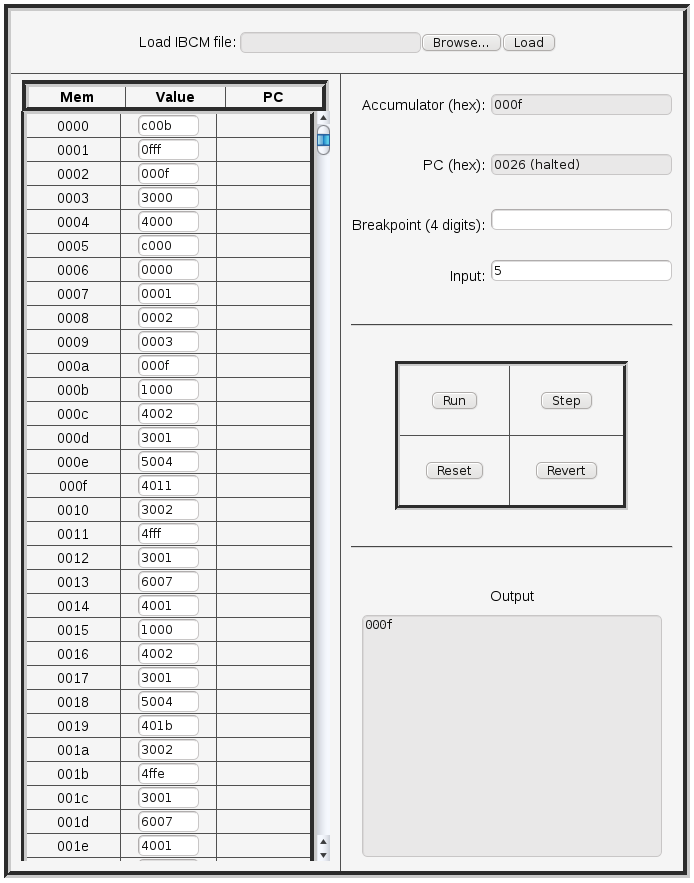
\includegraphics[width=3.25in]{ibcm/www-screen-shot.png}
\caption{Web-based IBCM interface}
\label{wwwinterface}
\vspace{-0.25in}
\end{wrapfigure}

To run an IBCM program, you can view the online simulator at
\url{http://libra.cs.virginia.edu/ibcm} \cite{ibcm-website}.  The
instructions listed in this section are also listed at that website.
An image of the online emulator is shown in Figure~\ref{wwwinterface}.

The simulator reads in text files, and proceeds to simulate the
result of an IBCM program execution.

To load a file, use the Browse button at the top of the simulator
page. Find the IBCM file, and click on the ``Load'' button. The format
of your program file is very rigid -- the first four characters of
each line are interpreted as a hexadecimal number. The number on the
first line is loaded into location zero, the next into location one
and so on. Characters after the first four on each line are ignored,
so you should use them to comment the code.  Blank lines are not
allowed, nor are lines that do not start with four hexadecimal digits
(i.e., no 'comment' lines).  An invalid file will either not load up
at all, or will load up gibberish.

The left side of the simulator lists all the memory locations (using
the hexadecimal address), the value in memory (if any), and the PC
(program counter) value. Note that any blank value field is
interpreted as'0000', as per the IBCM specification. When first
loaded, the simulator may uninitialized values blank to increase
readability.

The value column consists of a series of text boxes, which allow you
to directly edit the values in memory. The simulator will read the
current memory location from the appropriate text box when executing an
instruction. You can undo any edits by using the Revert button,
described below. The IBCM simulator does not check to ensure that your
entered values are valid~-- it is up to the user to do this. Note that
all hexadecimal values must be 4 digits (i.e. '0000', not '0'), or
else the simulator may not function correctly. Be sure to read the
section about crashing browsers and losing your work, below. There is
no way to save your edited work -- you will need to copy the changes
by hand. This is party due to a browser limitation, and partly due to
the fact that memory editing is meant to be a debugging tool, not a
means to write entire IBCM programs from scratch.

The 'PC' column lists the current value of the program counter. It can
have three values. Normally, it will have a left pointing arrow
('$<$-'), which indicates the next instruction that will be executed.
If the simulator is waiting for input, it will have a capital 'I' (for
Input) next to the input instruction that is currently awaiting a
value~-- and the ``Input'' text on the right side will blink. Lastly,
if the program has halted, then a capital 'H' (for Halt) will be
displayed next to the halt instruction that was executed.

On the right side, the values of the accumulator and program counter
are listed, both in hexadecimal notation. As mentioned above, the PC
field will also display, on the left side next to the hexadecimal
address, if the simulator is awaiting input or is halted. The Input
box is used to read in user input when a program requests it. When the
simulator is waiting for input, it will flash the 'Input' text. In
addition, the simulator will specify which type of input is being
requested: 'hex' or 'asc' for hexadecimal or ASCII input,
respectively. Note that for entering a hexadecimal value, you do not
need to enter all 4 digits: i.e., you can enter '12' instead of
'0012'. This is distinctly different that editing memory locations
(you have to enter all 4 digits for those). If you enter multiple
characters for ASCII input, it will only read in the first one.

Below this are four buttons. Two control execution: Run, which will
start a program executing, and Step, which will execute a single
instruction. Note that Run will execute until either a halt command is
reached, or until an input command is reached. The other two buttons
control the resetting of the IBCM program. The Reset button will reset
the PC and accumulator, in effect allowing the program to run again.
It will not, however, modify any memory locations. The Revert button
will do what a Reset does, but will also revert the memory locations
to what they were when the file was last loaded; it does not load the
file from disk again. Thus, if you have edited any of the memory
locations (or the IBCM program has modified them), then those changes
will be erased on a Revert, but not on a Reset. Note that a Revert
will not modify memory addresses outside the range that was loaded
(i.e. any 'blank' values).

Any output is displayed in the text area below these buttons. Each
output command prints the value (hexadecimal or ASCII character) on a
separate line.

A few notes:

\begin{itemize}

\item You will notice a slight delay when loading the simulator page.
  This is due to the fact that a number of scripts are run when the
  page loads (to initialize the memory table of 4096 elements, for
  example), and this takes a bit of time. How long this takes is
  determined by how fast a computer it is running on, as the scripts
  are run on the client side.

\item Upon entering input, hitting Enter is considered the same as
  hitting the Run button again. If you only want to execute a single
  instruction after an input, you must click on the Step button.

\item The simulator does minimal error checking with the input from
  the keyboard during program execution -- it is the user's
  responsibility to ensure that the input is properly formatted. The
  only error checking that is done is to ensure that a non-empty
  string was entered (if it was, then the simulator waits for more
  input).

\item Because of the limitations of threads running in web browsers,
  there is no way to terminate a program that is stuck in an infinite
  (or very long) loop -- the browser will not allow a polling
  (checking) to see if a Stop button was pressed, for example. Some
  browsers will pause the script after a minute or so of execution,
  and ask if the user wants to continue. Alternatively, you can close
  the web browser and restart. Note that this means if you have edited
  any of the memory locations, and your browser hangs or is restarted,
  you will lose any and all changes you have made to the memory
  locations!

\item The simulator page is a PHP script, which means that it will not
  work if you are viewing it as a local file (if the beginning of your
  URL is ``file://'' instead of ``http://''), or if the web server
  hosting this page does not have PHP installed (this latter
  restriction includes UVa's Collab web server).

\item Browser compatibility: It has been tested in Internet Explorer
  under Windows, Safari under Mac OS X, and Firefox under Windows, Mac
  OS X, and Ubuntu Linux. Note that the display of the changing of the
  values as the simulation is run (the PC, memory values, etc.) will
  only work on some browser / operating system combinations (Firefox,
  in particular, works well for this). The other browsers will have
  the same end state after the program is run, but will not animate
  the execution of the IBCM program when 'Run' is pressed (the 'Step'
  command will still animate each step).

\item The format of your program file is very rigid~-- the first four
  characters of each line are interpreted as a hexadecimal number. The
  number on the first line is loaded into location zero, the next into
  location one and so on. Characters after the first four on each line
  are ignored, so you should use them to comment the code; example
  code will be discussed in class.

\item When you execute a {\tt halt}, the simulator will halt with the PC
  pointing at the {\tt halt}.

\end{itemize}

\section{Writing IBCM Programs}

\subsection{Complex control structures}

\begin{wrapfigure}{r}{0.31\textwidth}
\vspace{-0.1in}
\begin{lstlisting}[caption={\bf if} pseudo code,backgroundcolor=\color{white},frame=trBL,linewidth=2in,xleftmargin=0.25in,label={IBCM-pseudo-code-if.lst}]
if ( B == 0 )
  S1;
else
S2
\end{lstlisting}
\vspace{0.25in}
\end{wrapfigure}

The control structures that we are familiar with in higher level
languages can be implemented in IBCM, albeit with a bit more effort.
Consider a typical pseudo code if-then-else conditional shown in
Listing~\ref{IBCM-pseudo-code-if.lst} to the right.

\begin{wrapfigure}{r}{0.31\textwidth}
\vspace{-0.4in}
\begin{lstlisting}[backgroundcolor=\color{white},frame=trBL,linewidth=2in,xleftmargin=0.25in,label={IBCM-code-if.lst},caption={IBCM {\bf if} code}]
load B
jmpe S1
S2: ...
jmp done;
S1: ...
done: ...
\end{lstlisting}
\vspace{-0.25in}
\end{wrapfigure}

The IBCM code for this conditional is shown in
Listing~\ref{IBCM-code-if.lst}.  Because we do not know many of the
required addresses (of variable B, or where S1 and S2 start in
memory), we have chosen to leave it in assembly format (i.e., using
opcodes) rather than provide machine code.

If we wanted to compare B to a different value, such as 5, we would
have to load B into the accumulator, subtract 5 from that, and then
perform a {\tt jmpe} or {\tt jmpl}.  This is illustrated further
below, when discussing the while loop.

Presumably, the ellipses at labels S1 and S2 would have some set of
IBCM opcodes to execute.

\begin{wrapfigure}{r}{0.31\textwidth}
\vspace{0.1in}
\begin{lstlisting}[backgroundcolor=\color{white},frame=trBL,linewidth=2in,xleftmargin=0.25in,label={IBCM-pseudo-code-while.lst},caption={{\bf while} pseudo code}]
while ( B >= 5 )
  S;
\end{lstlisting}
\vspace{0.25in}
\end{wrapfigure}

Loops are also easily converted to IBCM.  Note that a {\tt for} loop
is just a {\tt while} loop, but with a statement performed before the
loop starts (the ``for init''), and a statement performed at the end
of each loop iteration (the ``for update'').  Consider a straight
forward while loop shown in Listing~\ref{IBCM-pseudo-code-while.lst}.

\begin{wrapfigure}{r}{0.31\textwidth}
\vspace{-0.7in}
\begin{lstlisting}[backgroundcolor=\color{white},frame=trBL,linewidth=2in,xleftmargin=0.25in,label={IBCM-code-while.lst},caption={IBCM {\bf while} code}]
loop: load B
sub five
jmpl done
S: ...
jmp loop
done: ...
\end{lstlisting}
\vspace{-0.5in}
\end{wrapfigure}

We cannot directly compare a variable to the value 5; we can only
compare it to zero via the {\tt jmpe} and {\tt jmpl} instructions.
Our IBCM code is shown in Listing~\ref{IBCM-code-while.lst}.

If $B<5$, then we want our loop to terminate.  If $B<5$, then $B-5<0$,
so we will execute a {\tt jmpl} to break out of the loop.  If $B=5$,
then $B-5=0$, and we will continue in the loop.

\subsection{General tips}

When writing IBCM programs, we recommend these steps:

\begin{enumerate}
\item Write the pseudo code first~-- or even actual code~-- to make
  sure your algorithm works as desired.  If you have a bug in the
  design of your algorithm, then you will never get your IBCM code to
  work.
\item Write the program using IBCM opcodes, so that it looks like
  assembly: {\tt add one}, {\tt store x}, etc.  Comment this clearly!
\item Trace this assembly code, by hand, from beginning to end.  It
  will be {\em far} easier to find a bug in your program in the
  assembly stage than in the hexadecimal code stage.
\item Finally, translate it to machine code, and run it in the
  simulator.
\end{enumerate}

We cannot stress enough how important it is to first make sure that
the algorithm works, then to write and trace the assembly versions of
the program.  Debugging hexadecimal machine code is not much fun.



\section{Example Programs}


We present a number of IBCM example programs to help you get
acquainted with the language.

\subsection{Summation}

\begin{wrapfigure}{r}{0.45\textwidth}
%\vspace{-0.25in}
\lstinputlisting[caption=C++ summation program,label={C++program1.lst},backgroundcolor=\color{white},frame=trBL,linewidth=3.2in,xleftmargin=0.25in,language=C++]{ibcm/summation.cpp}
\vspace{-0.25in}
\end{wrapfigure}

The first program will compute the sum of the integers 1 through $n$,
where $n$ is read from the keyboard; the resulting sum is printed to
the screen. The program then halts after printing the sum.  The C++
code for the program is shown in Listing~\ref{C++program1.lst}~-- this is
presented to help show the conversion to IBCM.

The IBCM program is shown in Listing~\ref{IBCM-summation-program.lst}.
Note that the only part of the program that the simulator reads in is
the first four characters on the line.  The rest of the line in the
text file is solely for comments.  The column headers shown in the
figure are heavily abbreviated to fit in the width of a column, but
are, in order: the actual 4 hexadecimal digit memory value, the
hexadecimal location (used for determining jump targets and variable
addresses), the label (used to refer to jump and variable targets),
the opcode (from Table~\ref{IBCMopcodes.tbl}), the target address (which
refers to a given label), and any English comments. Note that the
column headers would not be in the input file; only the IBCM
hexadecimal instructions.  They are included in the listing for
clarity.

\begin{figure}[h]
\lstinputlisting[caption=IBCM summation program,label={IBCM-summation-program.lst},backgroundcolor=\color{white},frame=trBL,linewidth=6in,xleftmargin=1in]{ibcm/summation.ibcm.txt}
\end{figure}

\subsection{Array usage}

\begin{wrapfigure}{r}{0.45\textwidth}
%\vspace{-0.2in}
\begin{lstlisting}[caption=Array index pseudo code,label={array-index-pseudo-code.lst},backgroundcolor=\color{white},frame=trBL,linewidth=3.2in,xleftmargin=0.25in]
read A
read N
s = 0
i = 0
while (i < N)
	s += a[i]
	i += 1
print s;
\end{lstlisting}
\vspace{-0.4in}
\end{wrapfigure}

For this program, we will compute the sum of the elements of an array,
print this sum on the screen, and then halt.  Note that the array is
just a series of sequential spots in memory; it could be part of the
program itself, or a series of data values after the program itself.
The address of the first element of the array and the size of the
array are to be read from the keyboard.

The pseudo code for this program is shown in
Listing~\ref{array-index-pseudo-code.lst}.  C++ does not easily allow
for reading in an array address (while technically possible, it is not
very practical), so a C++ version of this program is not as useful as
a pseudo code version.

The IBCM code is shown in Listing~\ref{IBCM-array-index-program.lst}.

\begin{figure}[h!]
\lstinputlisting[caption=IBCM array index program,label={IBCM-array-index-program.lst},backgroundcolor=\color{white},frame=trBL,linewidth=6.8in,xleftmargin=0.25in]{ibcm/array-index.ibcm.txt}
\end{figure}

A quick note before the full analysis.  Notice that addresses 08
and 09 are blank~-- this was done to leave space for additional
variables.  If one has to add a variable into the program later,
shifting all of the successive instructions down is a frustrating
task, as all the addresses (of the jump targets, etc.)  need to be
shifted as well. So we left a few blank lines in case we needed
additional variables later on.

The challenging part of this program is the array subscripting.  In
our pseudo code~-- and in most programming languages~-- we use a syntax
such as {\tt a[i]}.  But the IBCM does not have any array subscripting
instruction~-- indeed, it cannot, as that requires two values (the
array base and the index). Thus, we have to {\em build} the
instruction to execute.

Our goal is to load the current sum (of the array elements processed
so far) into the accumulator, execute the instruction to add the
current {\tt a[i]} to the accumulator, and store that back into the
sum variable.  This is done in instructions 19, 1a, and 1b:
instruction 19 loads the current sum into the accumulator, instruction
1a is our special instruction that adds {\tt a[i]} to the accumulator
(how this works is next), and instruction 1b stores the updated result
back into the sum variable (address 002).

Thus, we want to create an instruction that will add a given {\tt
  a[i]} to the accumulator.  So we know it will be an add instruction
(opcode of 5).  The address that we want to add to the accumulator is
the array base plus the index.

For example, if the array starts at address 100, and we are trying to
add the value at index 5 of the array, our instruction would have
opcode of 5 (an add instruction), and address 105 (100 for the array
start plus 5 for the current index).  Thus, our instruction would be
5105.

To create this during the program execution, we start with 5000, which
sets the opcode of the instruction to the correct value for an add
instruction.  This is done in instruction 15, which is a load of the
{\tt adit} variable (address 007), which has value 5000.  To this
value of 5000 we add the array base (instruction 16) and then the
index (instruction 17).  Instruction 18 then stores that instruction
at the appropriate address (address 1a), overwriting the {\tt nop}
that is there with our updated instruction.  Once the current sum is
loaded (instruction 19), our custom instruction is executed
(instruction 1a), followed by the sum being stored back into memory
(instruction 1b).


\subsection{Recursive multiplication}

The next program computes the product of two numbers, $x$ and $y$,
through a recursive multiplication subroutine that uses only addition.
Both $x$ and $y$ are read from the keyboard, and the resulting product
is printed to the screen. The IBCM version is just over 100 lines of
opcodes.

\begin{wrapfigure}{r}{0.45\textwidth}
\vspace{-0.15in}
\lstinputlisting[backgroundcolor=\color{white},frame=trBL,linewidth=3in,xleftmargin=0.25in,language=C++,label={C++-multiplication-program.lst},caption={C++ multiplication program}]{ibcm/mult.cpp}
\vspace{-0.4in}
\end{wrapfigure}

The C++ code for the multiplication program can be seen in
Listing~\ref{C++-multiplication-program.lst}.  We did not create a
tail recursive {\tt multiply()} routine, as the IBCM compiler and
language is (intentionally) far too simple to optimize for tail
recursion.

This IBCM program creates a stack similar to x86: the stack starts at
the end of addressable memory, and grows downward.  An activation
record is created for each recursive call, which consists of the two
parameters and the return address~-- other fields typically in an
activation record (e.g., backup of registers) are not necessary in
IBCM.  The {\tt brl} instruction was used to allow for subroutine
calls~-- the return address is saved in the accumulator, and is stored
on the stack immediately upon subroutine activation.  We were able to
run the program with the second parameter (which is decremented in
each recursive call) set as high as 1,243 (0x4db), beyond which point
IBCM runs out of available memory for the stack.

This recursive multiplication program is beyond what we would expect
of a student to be able to program after a one-week introduction to
IBCM.  However, it is very illustrative of two important points about
IBCM.  One is that complex functionalities (such as multiplication)
can be achieved by using only the simple capabilities available in
IBCM (such as addition).  The other is that subroutines are fully
realizable in IBCM.

This program is shown in
Listings~\ref{IBCM-multiplication-program-pt1.lst} and
\ref{IBCM-multiplication-program-pt2.lst}.  Note that the only part of
the program that the simulators read in is the first four characters
on the line.  The rest of the line in the text file is solely for
comments.  The column headers and extra blank lines for comments are
shown in the diagram for clarity, but would not be included in the
IBCM source code file.

\begin{figure}
\lstinputlisting[caption={IBCM multiplication program, part 1},label={IBCM-multiplication-program-pt1.lst},backgroundcolor=\color{white},frame=trBL,linewidth=7.05in,xleftmargin=0.15in]{ibcm/multiplication-pt1.ibcm.txt}
\end{figure}

\begin{figure}
\lstinputlisting[caption={IBCM multiplication program, part 2},label={IBCM-multiplication-program-pt2.lst},backgroundcolor=\color{white},frame=trBL,linewidth=7.05in,xleftmargin=0.15in]{ibcm/multiplication-pt2.ibcm.txt}
\end{figure}

\section{Turing Completeness}

We were conflicted as to how much to discuss about Turing completeness
in this chapter.  IBCM is similar to a Random Access Stored Program
(RASP) machine \cite{wikipedia:rasp}, which is itself Turing complete,
so it is perhaps not surprising that IBCM is also Turing complete.
However, we felt that breaking down a complex task (a Turing machine
simulator) and programming it into IBCM was a worthwhile task to
discuss, as it emphasizes a primary design goal of IBCM~-- that
you can take any algorithm and write it in IBCM.

\begin{figure}[h]
\centering
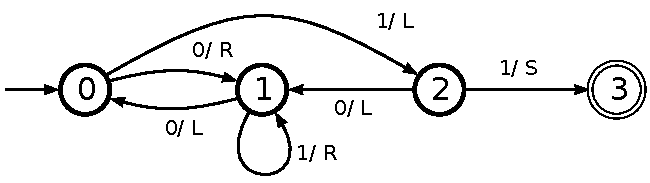
\includegraphics[width=4in]{ibcm/ibcm-automata.pdf}
\caption{Four state Busy Beaver automaton}
\label{BusyBeaverAutomaton}
\end{figure}

Obviously, no physical computer with a finite amount of memory can be
truly Turing complete.  Thus, we will instead show that the IBCM
computational model is Turing complete.

We define the {\em IBCM computational model} as the same IBCM computer
defined above, but allowing any sized integer to be held in a single
memory location, as well as having an infinite amount of memory.
Thus, other fields that make up part of a given instruction, such as
the 'address' or 'count' fields (see
Figure~\ref{IBCMInstructionFormat}), can also hold any size integer.

Given this model of computation, we will show how to simulate a Turing
machine in IBCM.  Hopcroft and Ullman \cite{HopcroftAndUllman} define
a Turing machine as a 7-tuple $M=\langle
Q,\Gamma,b,\Sigma,\delta,q_0,F \rangle$ where:

\begin{itemlist}
\item $Q$ is a finite set of states
\item $\Gamma$ is the finite set of allowable tape symbols
\item $b \in \Gamma$ is the blank symbol
\item $\Sigma \subseteq \Gamma \setminus {b}$ is the set of input symbols
\item $\delta : Q \times \Gamma \rightarrow Q \times \Gamma \times \{L,R\}$ is the transition function
\item $q_0 \in Q$ is the initial state
\item $F \subseteq Q$ is the set of final states
\end{itemlist}

We will make two modifications to the above definition, to allow for
ease of implementation in IBCM.  We will allow a no-shift transition
of $S$ (in addition to $L$ and $R$), which will not move the tape.
The Turing machine programs allowed by the no-shift are equivalent to
the ones described above \cite{wikipedia:turingmachine}. Furthermore,
we will define $f$, a single final state, which all states in $F$ move
to on a no-shift transition.

To represent the transition functions in IBCM, we will represent state
$q \in Q$ and symbol $\Sigma \in \Gamma$ each as a (16-bit) word in
IBCM.  Thus, states and symbols will be a single integer each.  While
this limits the number of states (and symbols) to $2^{16}=65,536$ in
our IBCM implementation, it is not limited in the formal IBCM
computational model.  Thus, one can encode any amount of states,
symbols, and transition functions into IBCM's memory.

To simulate a Turing machine, we will define an arbitrary memory
location to represent the current state of the Turing machine, and
another arbitrary memory location to contain the current address of
the head of the tape.  The transition function quintuples, $\delta$,
will start at a specific (but arbitrary) memory address, take up five
words each, and will contain the five parts listed above
$(Q,\Gamma,Q,\Gamma,\{L,R,S\})$.  The tape itself will start at
different arbitrary memory location.  Furthermore, we define a initial
state $q_0$ and a (single) final state $f$.  The blank symbol $b$ will
be an arbitrary value, such as -1 (0xffff in 16-bit 2's complement
integer).

Any Turing machine that requires a significant amount of tape will
need to be a one-way tape Turing machine, as the program code and
state transitions will lie at a lower address than the initial head
position.  Thus, only a finite amount of tape space is available in
the lower memory address direction.  The particular automaton example
that we provide, below, uses a two-way tape, but that is because we
know the finite amount of tape space necessary.  Note that one-way
tape Turing machines are equivalent in computational power to two-way
tape Turing machines \cite{HopcroftAndUllman}.

What is needed, then, is an IBCM program that will iterate through the
following steps:

\begin{itemlist}
\item Read the current state $s$, initially set to the start state.
  If the current state is the (single) final state, then exit.
\item Read the current head position.
\item Read the current input symbol $t$ at the head position
\item Search the list of transition functions until the appropriate
  one is found, based on the current state $s$ and the input symbol
  $t$.
\item Perform the action specified in the transition function by
  updating the state $s$, writing the specified symbol to the tape
  position, and then moving the tape left or right (or, on an $S$, not
  at all).
\end{itemlist}

We have developed such a program, described here.  The full listing of
the program is available online \cite{ibcm-website}.  The program
consists of 67 IBCM commands, and 15 variables~-- note that numeric
constants are considered variables in an IBCM program.  This program
only used half of the instructions: {\tt halt}, {\tt load}, {\tt
  store}, {\tt add}, {\tt sub}, {\tt nop}, {\tt jmp}, and {\tt jmpe}.

To test the Turing machine, we choose a four state Busy Beaver
automaton, which is described in more detail in the Wikipedia page on
Turing machine examples \cite{wikipedia:turingmachineexamples}.  The
Mea\-ly machine finite automaton is shown in
Figure~\ref{BusyBeaverAutomaton}.  For each transition, the input
symbol (0 or 1) is shown, along with the tape direction to move ($L$,
$R$, or $S$).  Note that in this automaton, upon each transition a 1
is written to the output tape; this is not shown in the figure to
improve clarity.  Also recall that the $S$
transition means to not move the tape, and is used only on the
transition to the final state.

Our implementation can utilize a two-way tape, although the tape in
one direction is finite.  We define memory address 1 as the current
state variable, and address 2 to store the location of the current
head position.  The transitions start at address 0x060, as our program
takes up 82 (or 0x052) instructions.  The states are numbered as per
the diagram in Figure~\ref{BusyBeaverAutomaton}, with 0 being the
initial state and 3 being the final state.  The program has constants
that specify both the initial and final states of the automaton.

% automaton figure goes here

The encoding of the automaton shown in
Figure~\ref{BusyBeaverAutomaton} is very straightforward.  The
transition from 2 to 1, executed on an input symbol of 0, will print 1
to the tape and then move the tape to the left.  The quintuple to be
encoded is $Q \times \Gamma \rightarrow Q \times \Gamma \times
\{L,R,S\}$.  The respective values for this transition are
$2,0,1,1,0$; we map the integer values $\{0,1,2\}$ to, respectively,
the transition directions $\{L,R,S\}$.


\section{Emulating IBCM in C++}

How might one write software to emulate an IBCM machine in C++?  A
switch statement with 16 cases, perhaps.  But how to decode the
instructions?

Let's assume we had to write a C++ program that could extract the
parts of an IBCM instruction.  How to do it?  Assume the instruction
is in an {\tt unsigned int x}.  One way to decode it is shown in
Listing~\ref{IBCM-decoding-instruction.lst}

\lstinputlisting[language=C++,backgroundcolor=\color{white},frame=trBL,linewidth=5.5in,xleftmargin=1.5in,label={IBCM-decoding-instruction.lst},caption={Decoding an IBCM instruction in C++}]{ibcm/emulating1.cpp}

What about encoding?  Assuming we have (unsigned ints) opcode,
ioshiftop and shiftcount, the decoding is shown in Listing~\ref{IBCM-encoding-instruction.lst}

\lstinputlisting[language=C++,backgroundcolor=\color{white},frame=trBL,linewidth=6.85in,xleftmargin=0.1in,label={IBCM-encoding-instruction.lst},caption={Encoding an IBCM instruction in C++}]{ibcm/emulating2.cpp}

This ends up being a rather frustrating program to write.  If the
instruction set being dealt with is more complicated than IBCM, as is
the case with x86 or MIPS instructions, then the above is very
difficult to do without any errors.

Listing~\ref{IBCM-encoding-data-structure.lst} shows a data structure
to make it easier.  While the IBCM is a big-Endian machine, the
following code may be running on a big or little-Endian machine.  The
{\tt BIG\_ENDIAN} and {\tt LITTLE\_ENDIAN} defines specify the
Endianness of the host machine.

\begin{figure}[h!]
\lstinputlisting[language=C++,backgroundcolor=\color{white},frame=trBL,linewidth=6.25in,xleftmargin=1in,label={IBCM-encoding-data-structure.lst},caption={C++ data structure to ease IBCM instruction encoding}]{ibcm/emulating3.cpp}
\end{figure}

We would use the data structure as shown in Listing~\ref{IBCM-encoding-data-structure-usage.lst}.

\begin{figure}[h!]
\lstinputlisting[language=C++,backgroundcolor=\color{white},frame=trBL,linewidth=6.25in,xleftmargin=1in,label={IBCM-encoding-data-structure-usage.lst},caption={Using the C++ data structure to encode IBCM instructions}]{ibcm/emulating4.cpp}
\end{figure}

\section{Pedagogy}

IBCM was originally developed at the University of Virginia to
complement our CS 3 course entitled {\em Program and Data
  Representation}, which is still taught today.  This course shows how
one represents both data and program code from high levels~-- such as
abstract data types~-- all the way down to the lowest (software)
level, which is the IBCM machine language.

IBCM allows students to easily make the mental connection between
assembly opcodes and the machine language that they get translated
into.  At the University of Virginia, we follow the presentation of
IBCM with a two-week introduction to x86 assembly language.  This
allows students to understand both machine language, as well as a
modern processor's assembly language (we use Intel x86), without
having to delve into the details of x86 machine language.

A specific design decision with IBCM was to include only basic
operations~-- for example, multiplication and division are not
included, but can be replicated by using repeated addition or
subtraction.  We wanted students to see that any program, no matter
how complicated, can be broken down into very simple instructions.
Indeed, this is the point of the concept of Turing machines, but they
are often not taught when students are first seeing machine language.

Students are exposed to a number of concepts during the IBCM module
that they often have not seen previously.  They become aware that in
both assembly language and machine language, data is untyped, and the
operations on the data determine the type~-- this is quite different
than the typed high-level programming languages to which they are
accustomed.  By this point in our course, students have been exposed
to how a 32-bit value can be interpreted either as a two's-complement
signed integer or an IEEE 754 floating point number.

Another concept taught through IBCM is self-modifying programs.  A
non-trivial IBCM program requires arithmetic on instructions~-- in
fact, only the first example program shown in
Listing~\ref{IBCM-summation-program.lst} did not use this feature.  Array indexing,
for example, requires starting with a {\tt load} or {\tt add}
instruction, and adding to that value both the base address of the
array and the current index.  This value is then stored in a memory
address which is shortly thereafter executed.  The second example
program provided to the students uses this feature.  While many
systems explicitly try to prevent self-modifying code, as that is an
exploit used by a significant amount of malware, it is still a concept
that the students should be familiar with.

The development of self-modifying IBCM programs leads to another
pedagogical goal of the course: the interplay between data and program
code.  Indeed, there is little difference between data and program
code, other than the values (obviously), and how it is interpreted
(and, in modern systems, what segment of an executable in which the
data is found).  This concept seems trivial to instructors, but is one
that students who have only programmed using high-level languages are
often unfamiliar with.

What IBCM does not teach, of course, is how binary machine
language instructions are executed on the processor.  Understanding of
this material is typically beyond all but senior-level undergraduate
courses; at many institutions, this is also outside the
standard computing curriculum.

\subsection{Materials Available}

We have developed and made available a wide range of materials for the
purpose of teaching the IBCM module.  The materials are all released
under various Creative Commons licenses.  They are available online
\cite{ibcm-website}, and consist of:

\begin{itemlist}
\item A PowerPoint slide set to introduce the concepts during a
  lecture-based course.  This 42 slide set takes about three 50-minute
  lectures to present.
\item A {\em Principles of Operation} document, which describes the
  IBCM computer and language, and how to write a program.
  It covers similar content to the lecture slides.
\item Sample programs, one of which was shown in
  Listing~\ref{IBCM-summation-program.lst}, above.  We also provide sample programs
  on array indexing, for example.  All the programs mentioned in this
  article are available online.
\item Sample student assignments, which require students to
  write additional IBCM programs beyond the sample programs provided.
  One of the assignments is to write a quine, or an IBCM program that
  will print itself out~-- the smallest quine produced is nine IBCM
  commands.
\item An online PHP/Javascript simulator, which is the primary way that
  the students program in IBCM.  This is shown above in
  Figure~\ref{wwwinterface}.  The PHP is used to allow loading of an
  IBCM program from a text file; the Javascript implements the IBCM
  simulator in the browser itself.  The simulator works across all
  major browsers on all major operating systems.
\item A C++-based command-line program, which can both compile and
  execute IBCM programs.  Not surprisingly, this is much faster than
  the online simulator.  This is particularly useful for automated
  compilation and execution of IBCM programs for grading, or for very
  long programs, such as the recursive multiply routine described
  above.
\end{itemlist}

Furthermore, a GUI-based tool for executing IBCM programs is available
separately \cite{jwelsh-ibcm}.
This tool allows for drag-and-drop loading of IBCM files into the
GUI, and compiles natively for each operating system.

% web interface image goes here

We very specifically have not developed an IBCM assembler, which would
take in the opcodes in an assembly language format and output
hexadecimal machine code.  The purpose of IBCM is to teach the
students machine language; given an IBCM assembler, this module ends
up being just a different assembly language for the students to learn.

\subsection{Related Work}

We are certainly not the first to propose a simplified machine
language as a pedagogical tool.  Andrew Tanenbaum's original 1984
text, {\em Structured Computer Organization}~-- now in its 5th
edition~-- presents the Mic-1 micro architecture and the Mac-1 machine
language \cite{538160}.  Indeed, the Mac-1 machine language has many
similarities with IBCM~-- this is not surprising, as there are many
common elements that must be present in all small instruction set
machine languages.  Further research in that decade presented
implementations of those languages \cite{54147,152757}.  The Mic-1
simulator, which is focused on assembly language, is available online
\cite{mic-1-website}.  Simulators for the Mac-1 machine language do
exist, but seem to be independently developed, and without a modern
set of implementation software.

A number of high quality simulators exist at the assembly level.
Pep/8 \cite{warford:2010:PMT:1734263.1734389,warford2009computer} is a
16-bit CISC architecture designed to teach assembly language concepts.
While it can be used for machine language~-- and can trace program
execution at the machine language level~-- the primary pedagogical
design is at the assembly language level. Another example is SPIM,
which is a full featured MIPS 32-bit simulator \cite{spim-website}.

Additional research on machine language simulators has often focused
on the register transfer level \cite{107081}, or is restricted to a
single client operating system \cite{199795}.

More recent research by Stone has focused on a similar machine
language implementation \cite{1189166}.  Although developed
independently, our research can be seen as an extension of Stone's, as
we add a number of additional aspects: significant pedagogical tools,
a fully downloadable package so this system can be used in any course,
a proof of Turing completeness, and a discussion of pedagogical
concerns.  

We are not aware of any machine language simulators that are available
with the set of modern tools that we present with IBCM.


\subsection{Results}

At the University of Virginia, this module is taught about half-way
through our CS3 course, which is where we teach data structures.  Our
CS1 and CS2 course are both in Java.  At this point in the CS3 course,
the students have learned to implement a number of data structures in
C++.  We introduce machine language using IBCM for one week, follow
that with two weeks of assembly programming (x86), and then return to
C++ for the remainder of the semester.  The lectures used to teach
IBCM typically take three 50-minute class periods.  This is followed
by an IBCM lab the following week.  All of the lecture slides and labs
are available online~\cite{ibcm-website}.

We have taught machine language using IBCM in our CS3 class for over a
decade here at the University of Virginia.  Over the years, student
reactions to IBCM have varied greatly.  With the usage of the modern
tool set presented in this article, those reactions have generally
been positive, as shown below While they often do not like being
constrained to such a limited set of instructions, they see the
purpose of learning machine language, and generally enjoy the IBCM
assignments.  We have found that the quality of the software tools is
directly related to student perception of IBCM~-- in the past, when
our IBCM simulator was less refined, student reaction was
significantly more negative.

Objective comparison with other programming languages, including
assembly language, are difficult due to the vast differences between
both the capabilities and the required learning curve.  We have
instead focused on subjective assessment.  In the most recent semester
in which IBCM was used (fall of 2010), six questions were asked of the
students.  All questions were asked on a Likert scale, where 1 means
strongly agree, 2 is agree, 3 is neutral, 4 is disagree, and 5 is
strongly disagree.  For all the questions, $n=89$.

The first two questions focused on how much the students felt they
learned from the IBCM module.  The middle two questions focused on the
ease of use and enjoyability.  And the last two questions focused on
how worthwhile this module was, both for this course and future courses.
The results are shown in Table~\ref{IBCM-survey-results.tbl}.

\begin{table}[h]
\centering
\begin{tabular}{|p{5in}|c|c|}  \hline
\bf Question & \bf Avg & \bf Stdev \\ \hline \hline
IBCM increased my understanding of the basics of machine language &
1.67 & 0.58 \\ \hline
IBCM increased my understanding of how computers work at a low level &
1.89 & 0.65 \\ \hline
IBCM was easy to use, once I got the hang of programming in it & 1.92
& 0.88 \\ \hline
I enjoyed learning IBCM & 2.01 & 0.98 \\ \hline
Considering what was taught, IBCM was a worthwhile module to have in
this course & 1.75 & 0.68 \\ \hline
IBCM should be used in future iterations of this course & 1.76 & 0.72
\\ \hline
\end{tabular}
\caption{IBCM survey results}
\label{IBCM-survey-results.tbl}
\end{table}

The results clearly show that the module was generally well received.
The lowest score, enjoyment of learning IBCM, still was in the 'agree'
category.

\section{Conclusions}

We have used IBCM for over a decade at the University of
Virginia in our CS3
class.  During that time, we have refined it into the pedagogical tool
presented here.  With the set of current pedagogical tools provided,
we have found it to be an effective means of teaching the basic
concepts of machine language without having to go into the complexity
of modern machine languages that is beyond the scope of a lower-level
undergraduate course.  All of the necessary materials are available
online for adoption at other institutions.



\chapter{32-bit x86 Assembly}

\begin{quotation}
\ldots
\end{quotation}

\noindent {\em This chapter was derived from a document written by Adam Ferrari and later updated by Alan Batson, Mike Lack, Anita
Jones, and Aaron Bloomfield}

\section{Introduction}

This small guide, in combination with the material covered in the
class lectures on assembly language programming, should provide enough
information to do the assembly language labs for this class. In this
guide, we describe the basics of 32-bit x86 assembly language
programming, covering a small but useful subset of the available
instructions and assembler directives. However, real x86 programming
is a large and extremely complex universe, much of which is beyond the
useful scope of this class. For example, there exists real (albeit
older) x86 code running in the world was written using the 16-bit
subset of the x86 instruction set. Using the 16-bit programming model
can be quite complex~-- it has a segmented memory model, more
restrictions on register usage, and so on. In this guide we'll
restrict our attention to the more modern aspects of 32-bit x86
programming, and delve into the instruction set only in enough detail
to get a basic feel for programming x86 compatible chips at the
hardware level.

\section{Registers}

Modern (i.e., 386 and beyond) x86 processors have eight 32-bit general
purpose registers, as depicted in
Figure~\ref{x86-register-diagram.fig}. The register names are mostly
historical in nature. For example, EAX used to be called the
``accumulator'' since it was used by a number of arithmetic
operations, and ECX was known as the ``counter'' since it was used to
hold a loop index. Whereas most of the registers have lost their
special purposes in the modern instruction set, by convention, two are
reserved for special purposes~-- the stack pointer (ESP) and the base
pointer (EBP).

\begin{figure}[h]
\begin{center}
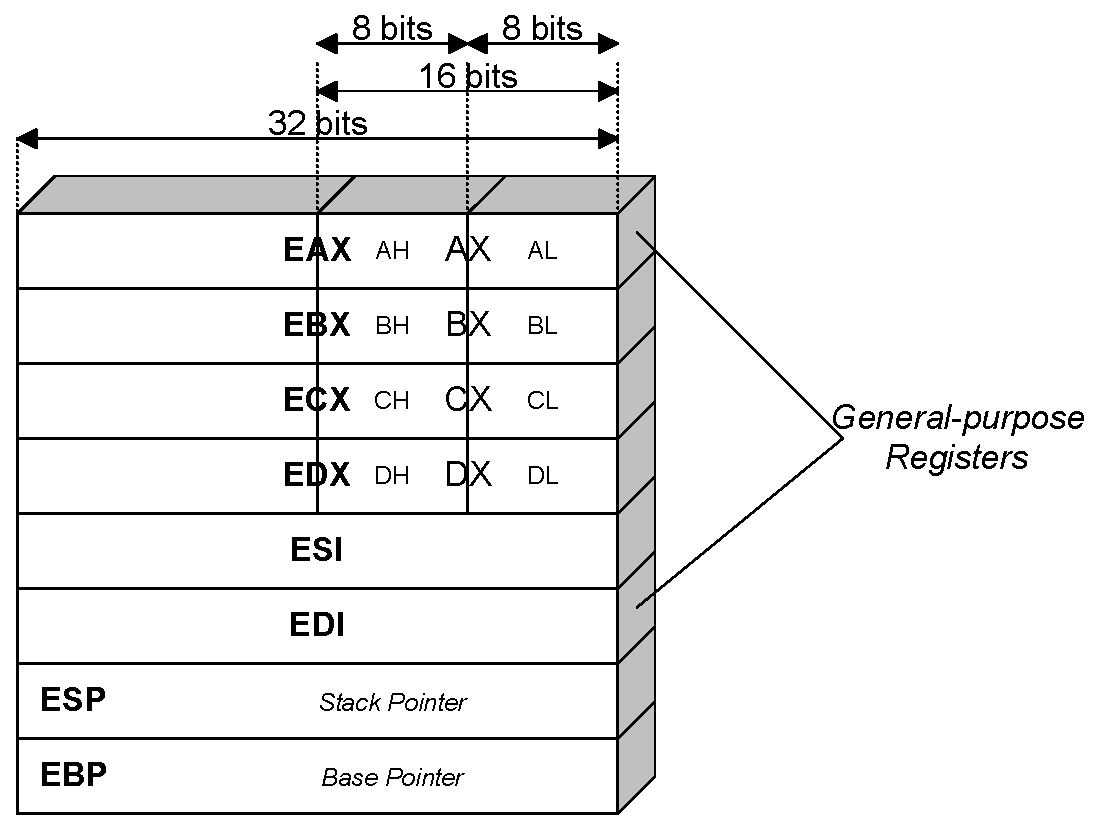
\includegraphics[width=4in]{x86-32bit/x86-register-diagram.pdf}
\end{center}
\caption{The x86 register set}
\label{x86-register-diagram.fig}
\end{figure}

In some cases, namely EAX, EBX, ECX, and EDX, subsections of the
registers may be used.  For example, the least significant 2 bytes of
EAX can be treated as a 16-bit register called AX.  The least
significant byte of AX can be used as a single 8-bit register called
AL, while the most significant byte of AX can be used as a single
8-bit register called AH. It is important to realize that these names
refer to the same physical register. When a two-byte quantity is
placed into DX, the update affects the value of EDX (in particular,
the least significant 16 bits of EDX). These ``sub-registers''
are mainly hold-overs from older, 16-bit versions of the instruction
set. However, they are sometimes convenient when dealing with data
that are smaller than 32-bits (e.g., 1-byte ASCII characters).

When referring to registers in assembly language, the names are not
case-sensitive. For example, the names EAX and eax refer to the same
register.

\section{Memory and Addressing Modes}

\subsection{Declaring Static Data Regions}

You can declare static data regions (analogous to global variables) in
x86 assembly using special assembler directives for this purpose.
Data declarations should be preceded by the .DATA directive. Following
this directive, the directives DB, DW, and DD can be used to declare
one, two, and four byte data locations, respectively. Declared
locations can be labeled with names for later reference - this is
similar to declaring variables by name, but abides by some lower level
rules. For example, locations declared in sequence will be located in
memory next to one another.  Some example declarations are depicted in
Listing~\ref{x86-declaring-memory-regions.lst}.

\begin{figure}[h]
\lstinputlisting[caption=Declaring x86 memory regions,label={x86-declaring-memory-regions.lst},backgroundcolor=\color{white},frame=trBL,linewidth=7in,xleftmargin=0in,language={[x86masm]Assembler}]{x86-32bit/code/memory-regions.s}
\end{figure}

The last example in Listing~\ref{x86-declaring-memory-regions.lst}
illustrates the declaration of an array.  Unlike in high level
languages where arrays can have many dimensions and are accessed by
indices, arrays in assembly language are simply a number of cells
located contiguously in memory. Two other common methods used for
declaring arrays of data are the TIMES directive and the use of string
literals. The TIMES directive tells the assembler to duplicate an
expression a given number of times. For example, the statement ``TIMES
4 DB 2'' is equivalent to ``2, 2, 2, 2''. Some examples of declaring
arrays are depicted in Listing~\ref{x86-declaring-arrays.lst}.

\begin{figure}[h]
\lstinputlisting[caption=Declaring x86 arrays in memory,label={x86-declaring-arrays.lst},backgroundcolor=\color{white},frame=trBL,linewidth=7in,xleftmargin=0in,language={[x86masm]Assembler}]{x86-32bit/code/declaring-arrays.s}
\end{figure}

\subsection{Addressing Memory}
\label{addressing-memory.sec}

Modern x86-compatible processors are capable of addressing up to
$2^{32}$ bytes of memory; that is, memory addresses are 32-bits wide.
For example, in Listings~\ref{x86-declaring-memory-regions.lst} and
\ref{x86-declaring-arrays.lst}, where we used labels to refer to memory
regions, these labels are actually replaced by the assembler with
32-bit quantities that specify addresses in memory. In addition to
supporting referring to memory regions by labels (i.e. constant
values), the x86 provides a flexible scheme for computing and
referring to memory addresses:

{\bf x86 Addressing Mode Rule}~-- Up to two of the 32-bit registers
and a 32-bit signed constant can be added together to compute a memory
address. One of the registers can be optionally pre-multiplied by 2,
4, or 8.

To see this memory addressing rule in action, we'll look at some
example mov instructions.  As we'll see later in
Section~\ref{data-movement-instructions.sec}, the {\tt mov} instruction
moves data between registers and memory.  This instruction has two
operands~-- the first is the destination (where we're moving data {\em
  to}) and the second specifies the source (where we're getting the
data {\em from}). Some examples of mov instructions using address
computations that obey the above rule are shown in
Listing~\ref{x86-valid-addressing-modes.lst}.

\begin{figure}[h]
\lstinputlisting[caption={Valid x86 addressing modes},label={x86-valid-addressing-modes.lst},backgroundcolor=\color{white},frame=trBL,linewidth=7in,xleftmargin=0in,language={[x86masm]Assembler}]{x86-32bit/code/valid-addressing-modes.s}
\end{figure}

Some examples of incorrect address calculations are shown in Listing~\ref{x86-invalid-addressing-modes.lst}.

\begin{figure}[h]
\lstinputlisting[caption={Invalid x86 addressing modes},label={x86-invalid-addressing-modes.lst},backgroundcolor=\color{white},frame=trBL,linewidth=7in,xleftmargin=0in,language={[x86masm]Assembler}]{x86-32bit/code/invalid-addressing-modes.s}
\end{figure}


\subsection{Size Directives}

In general, the intended size of the of the data item at a given memory address can be inferred
from the assembly code instruction in which it is referenced. For example, in all of the above
instructions, the size of the memory regions could be inferred from the size of the register operand~-- when we were loading a 32-bit register, the assembler could infer that the region of memory
we were referring to was 4 bytes wide. When we were storing the value of a one byte register to
memory, the assembler could infer that we wanted the address to refer to a single byte in memory.
However, in some cases the size of a referred-to memory region is ambiguous. Consider the instruction {\tt mov [ebx], 2}.


Should this instruction move the value 2 into the single byte at
address EBX? Perhaps it should move the 32-bit integer representation
of 2 into the 4-bytes starting at address EBX. Since either is a valid
possible interpretation, the assembler must be explicitly directed as
to which is correct.  The size directives {\tt BYTE PTR}, {\tt WORD
  PTR}, and {\tt DWORD PTR} serve this purpose. For examples, see
Listing~\ref{x86-size-directives.lst}.

\begin{figure}[h]
\lstinputlisting[caption={x86 size directive usage},label={x86-size-directives.lst},backgroundcolor=\color{white},frame=trBL,linewidth=7in,xleftmargin=0in,language={[x86masm]Assembler}]{x86-32bit/code/size-directives.s}
\end{figure}


\section{Instructions}

Machine instructions generally fall into three categories: data movement, arithmetic/logic,
and control-flow. In this section, we will look at important examples of x86 instructions from
each category. This section should not be considered an exhaustive list of x86 instructions, but
rather a useful subset.

In this section, we will use the following notation:

\begin{itemlist}
\item $<$reg32$>$ - means any 32-bit register described in Section 2, for example, ESI.
\item $<$reg16$>$ - means any 16-bit register described in Section 2, for example, BX.
\item $<$reg8$>$ - means any 8-bit register described in Section 2, for example AL.
\item $<$reg$>$ - means any of the above.
\item $<$mem$>$ - will refer to a memory address, as described in Section~\ref{addressing-memory.sec}, for example {\tt [EAX]}, or
{\tt [var+4]}, or {\tt DWORD PTR [EAX+EBX]}.
\item $<$con32$>$ - means any 32-bit constant.
\item $<$con16$>$ - means any 16-bit constant.
\item $<$con8$>$ - means any 8-bit constant.
\item $<$con$>$ - means any of the above sized constants.
\end{itemlist}

\subsection{Data Movement Instructions}
\label{data-movement-instructions.sec}

\asminstructionsummary{mov}
{mov $<$reg$>$,$<$reg$>$\newline mov $<$reg$>$,$<$mem$>$\newline mov $<$mem$>$,$<$reg$>$\newline mov $<$reg$>$,$<$const$>$\newline mov $<$mem$>$,$<$const$>$}
{The mov instruction moves the data item referred to by its second
  operand (i.e.  register contents, memory contents, or a constant
  value) into the location referred to by its first operand (i.e. a
  register or memory). While register-to-register moves are possible,
  direct memory-to-memory moves are not. In cases where memory
  transfers are desired, the source memory contents must first be
  loaded into a register, then can be stored to the destination memory
  address.}
{mov eax, ebx \linebreak mov BYTE PTR [var], 5 }
{; transfer ebx to eax\linebreak; store the value 5 into the byte at\linebreak; memory location ``var''}
{2.2in}{3.5in}

\asminstructionsummary{push}
{push $<$reg32$>$\newline push $<$mem$>$\newline push $<$con32$>$}
{The push instruction places its operand onto the top of the hardware supported
stack in memory. Specifically, push first decrements ESP by 4, then places its
operand into the contents of the 32-bit location at address [ESP]. ESP (the stack
pointer) is decremented by push since the x86 stack grows down~-- i.e. the stack
grows from high addresses to lower addresses.}
{push eax\newline push [var]}
{; push the contents of eax onto the stack\newline
; push the 4 bytes at address ``var'' onto stack}
{1in}{4.7in}

\asminstructionsummary{pop}
{pop $<$reg32$>$\newline pop $<$mem$>$}
{The pop instruction removes the 4-byte data element from the top of
  the hardware supported stack into the specified operand (i.e.
  register or memory location). Specifically, pop first moves the 4
  bytes located at memory location [ESP] into the specified register or
  memory location, and then increments SP by 4.}
{pop edi \newline pop [ebx]}
{; pop the top element of the stack into EDI.\newline
; pop the top element of the stack into memory at\newline
; the four bytes starting at location EBX.}
{1in}{4.7in}

\asminstructionsummary{lea}
{lea $<$reg32$>$,$<$mem$>$}
{The lea instruction places the address specified by its second
  operand into the register specified by its first operand. Note, the
  contents of the memory location are not loaded~-- only the effective
  address is computed and placed into the register.  This is useful
  for obtaining a ``pointer'' into a memory region.}
{lea eax, [var]\newline lea edi, [ebx+4*esi]}
{; the address of ``var'' is placed in EAX \newline
; the value EBX+4*ESI is placed in EDI}
{1.85in}{3.85in}

\subsection{Arithmetic and Logic Instructions}

\asminstructionsummary{add, sub}
{add $<$reg$>$,$<$reg$>$ \hspace{0.5in} sub $<$reg$>$,$<$reg$>$ \newline
add $<$reg$>$,$<$mem$>$ \hspace{0.5in} sub $<$reg$>$,$<$mem$>$ \newline
add $<$mem$>$,$<$reg$>$ \hspace{0.5in} sub $<$mem$>$,$<$reg$>$ \newline
add $<$reg$>$,$<$con$>$ \hspace{0.5in} sub $<$reg$>$,$<$con$>$ \newline
add $<$mem$>$,$<$con$>$ \hspace{0.5in} sub $<$mem$>$,$<$con$>$}
{The add instruction adds together its two operands, storing the
  result in its first operand. Similarly, the sub instruction
  subtracts its second operand from its first.  Note, whereas both
  operands may be registers, at most one operand may be a memory
  location.}
{add eax, 10\newline 
sub [var], esi\newline\newline\newline
add BYTE PTR [var], 10}
{; add 10 to the contents of EAX. \newline
; subtract the contents of ESI from \newline
; the 32-bit integer stored at \newline
; memory location ``var''.\newline
; add 10 to the single byte stored\newline
; at memory address ``var''.\newline}
{2.2in}{3.5in}

\asminstructionsummary{inc, dec}
{inc $<$reg$>$ \hspace{0.5in} dec $<$reg$>$\newline
inc $<$mem$>$ \hspace{0.5in} dec $<$mem$>$}
{The inc instruction increments the contents of its operand by one,
  and similarly dec decrements the contents of its operand by one.}
{dec eax \newline inc DWORD PTR [var]}
{; subtract one from the contents of EAX. \newline
; add one to the 32-bit integer stored at \newline
; memory location ``var''.}
{1.8in}{3.9in}

\asminstructionsummary{imul}
{imul $<$reg32$>$,$<$reg32$>$\newline
imul $<$reg32$>$,$<$mem$>$\newline
imul $<$reg32$>$,$<$reg32$>$,$<$con$>$\newline
imul $<$reg32$>$,$<$mem$>$,$<$con$>$}
{The imul instruction has two basic formats: two-operand (first two
syntax listings above) and three-operand (last two syntax listings
above).  The two-operand form multiplies its two operands together and
stores the result in the first operand. The result (i.e., first)
operand must be a register.  The three operand form multiplies its
second and third operands together and stores the result in its first
operand. Again, the result operand must be a register.  Furthermore,
the third operand is restricted to being a constant value.}
{imul eax, [var]\newline\newline\newline
imul esi, edi, 25}
{; multiply the contents of EAX by the \newline
; 32-bit contents of the memory location \newline
; ``var''. Store the result in EAX.\newline
; multiply the contents of EDI by 25. \newline
; Store the result in ESI.}
{1.8in}{3.9in}

\asminstructionsummary{idiv}
{idiv $<$reg32$>$\newline
idiv $<$mem$>$}
{The idiv instruction is used to divide the contents of the 64 bit
  integer EDX:EAX (constructed by viewing EDX as the most significant
  four bytes and EAX as the least significant four bytes) by the
  specified operand value. The quotient result of the division is
  stored into EAX, while the remainder is placed in EDX. This
  instruction must be used with care. Before executing the
  instruction, the appropriate value to be divided must be placed into
  EDX and EAX. Clearly, this value is overwritten when the idiv
  instruction is executed.}
{idiv ebx \newline\newline\newline idiv DWORD PTR [var]}
{; divide the contents of EDX:EAX by the \newline
; contents of EBX. Place the quotient \newline
; in EAX and the remainder in EDX.\newline
; same as above, but divide by the \newline
; 32-bit value stored at memory \newline
; location ``var''.}
{1.9in}{3.8in}

\asminstructionsummary{and, or, xor}
{and $<$reg$>$,$<$reg$>$ \hspace{0.25in} or $<$reg$>$,$<$reg$>$ \hspace{0.25in} xor $<$reg$>$,$<$reg$>$ \newline
and $<$reg$>$,$<$mem$>$ \hspace{0.25in} or $<$reg$>$,$<$mem$>$ \hspace{0.25in} xor $<$reg$>$,$<$mem$>$ \newline
and $<$mem$>$,$<$reg$>$ \hspace{0.25in} or $<$mem$>$,$<$reg$>$ \hspace{0.25in} xor $<$mem$>$,$<$reg$>$ \newline
and $<$reg$>$,$<$con$>$ \hspace{0.25in} or $<$reg$>$,$<$con$>$ \hspace{0.25in} xor $<$reg$>$,$<$con$>$ \newline
and $<$mem$>$,$<$con$>$ \hspace{0.25in} or $<$mem$>$,$<$con$>$ \hspace{0.25in} xor $<$mem$>$,$<$con$>$}
{These instructions perform the specified logical operation (logical
bitwise and, or, and exclusive or, respectively) on their operands,
placing the result in the first operand location.}
{and eax, 0fH \newline xor edx, edx}
{; clear all but the last 4 bits of EAX. \newline ; set the contents of EDX to zero.}
{1.7in}{4in}

\asminstructionsummary{not}
{not $<$reg$>$ \newline not $<$mem$>$}
{Performs the logical negation of the operand contents (i.e., flips all bit values).}
{not BYTE PTR [var]}
{; negate all bits in the byte at the \newline ; memory location ``var''.}
{1.7in}{4in}

\asminstructionsummary{neg}
{neg $<$reg$>$ \newline neg $<$mem$>$}
{Performs the arithmetic (i.e., two's complement) negation of the operand contents.}
{neg eax \newline neg [var]}
{; negate the contents of EAX. \newline ; negate the contests of ``var''}
{1.4in}{4.3in}

\asminstructionsummary{shl, shr}
{shl $<$reg$>$,$<$con8$>$ \hspace{0.5in} shr $<$reg$>$,$<$con8$>$\newline
shl $<$mem$>$,$<$con8$>$ \hspace{0.5in} shr $<$mem$>$,$<$con8$>$\newline
shl $<$reg$>$,cl \hspace{0.92in} shr $<$reg$>$,cl\newline
shl $<$mem$>$,cl \hspace{0.92in} shr $<$mem$>$,cl}
{These instructions shift the bits in their first operand's contents
  left and right ({\tt shl} and {\tt shr}, respectively), padding the
  resulting empty bit positions with zeros. The shifted operand can be
  shifted up to 31 places. The number of bits to shift is specified
  by the second operand, which can be either an 8-bit constant or the
  register CL. In either case, shifts counts of greater then 31 are
  performed modulo 32.}
{shl eax 5 \newline\newline shr [var] 3}{; shift the contents of eax left by 5 bit \newline ; positions \newline ; shift the contents of ``var'' right by 3 \newline ; bit positions}{1.4in}{4.3in}

\subsection{Control Flow Instructions}

In this section, we will refer to labeled locations in the program
text as $<$label$>$. Labels can be inserted anywhere in x86 assembly
code text by entering a label name followed by a colon. For example,
consider the code fragment in Listing~\ref{x86-labeled-code-location.lst}.
The second instruction in this code fragment is labeled ``begin''.
Elsewhere in the code, we can refer to the memory location that this
instruction is located at in memory using the more convenient symbolic
name ``begin'' instead of having to refer to the memory address as an
integer.

\begin{figure}[h]
\lstinputlisting[caption={x86 labeled code location},label={x86-labeled-code-location.lst},backgroundcolor=\color{white},frame=trBL,linewidth=4.75in,xleftmargin=2.25in,language={[x86masm]Assembler}]{x86-32bit/code/labeled-code-location.s}
\end{figure}


\asminstructionsummary{jmp}
{jmp $<$label$>$}
{Transfers program control flow to the instruction at the memory
  location indicated by the operand.}
{jmp begin}{; jumps to the ``begin'' label}
{1.5in}{3.7in}

\asminstructionsummary{jCC}
{je $<$label$>$ ; Jump when equal\newline
jne $<$label$>$ ; Jump when not equal\newline
jz $<$label$>$ ; Jump when last result was zero\newline
jg $<$label$>$ ; Jump when greater than\newline
jge $<$label$>$ ; Jump when greater than or equal to\newline
jl $<$label$>$ ; Jump when less than\newline
jle $<$label$>$ ; Jump when less than or equal to}
{These instructions are conditional jumps that are based on the status
  of a set of {\bf condition codes} that are stored in a special
  register called the {\em machine status word}. The contents of the
  machine status word include information about the last arithmetic
  operation performed. For example, one bit of this word indicates if
  the last result was zero. Another indicates if the last result was
  negative.  Based on these condition codes, a number of conditional
  jumps can be performed. For example, the jz instruction performs a
  jump to the specified operand label if the result of the last
  arithmetic operation (e.g. add, sub, etc.) was zero. Otherwise,
  control proceeds to the next instruction in sequence after the jz.
  These conditional jumps are the underlying support needed to
  implement high-level language features such as ``if'' statements and
  loops (e.g. ``while'' and ``for''). \vspace{6pt}\newline
  A number of the conditional branches are given names that are
  intuitively based on the last operation performed being a special
  compare instruction, cmp (see below).  For example, conditional
  branches such as jle and jne are based on first performing a cmp
  operation on the desired operands.}
{cmp eax, ebx \newline jle done}
{; if the contents of eax are less than or \newline
; equal to the contents of EBX, jump to the \newline
; code location labeled ``done''.}
{1.4in}{4.3in}

\asminstructionsummary{cmp}
{cmp $<$reg$>$,$<$reg$>$\newline
cmp $<$reg$>$,$<$mem$>$\newline
cmp $<$mem$>$,$<$reg$>$\newline
cmp $<$reg$>$,$<$con$>$\newline
cmp $<$mem$>$,$<$con$>$}
{Compares the two specified operands, setting the condition codes in
  the machine status word appropriately. In fact, this instruction is
  equivalent to the sub instruction, except the result of the
  subtraction is discarded.}
{cmp DWORD PTR [var], 10\newline jeq loop}
{; if the 4 bytes stored at memory\newline
; location ``var'' equal the 4-byte\newline
;  integer value 10, then jump to the\newline
; code location labeled loop}
{2.2in}{3.5in}

\asminstructionsummary{call}
{call $<$label$>$}
{This instruction implements a subroutine call that operates in
cooperation with the subroutine return instruction, ret, described
below. This instruction first pushes the current code location onto
the hardware supported stack in memory (see the push instruction for
details), and then performs an unconditional jump to the code location
indicated by the label operand. The added value of this instruction
(as compared to the simple jmp instruction) is that it saves the
location to return to when the subroutine completes.}
{call my\_subroutine}
{; jumps to the ``my\_subroutine'' label, \newline
; pushing the return address onto the \newline
; stack}
{1.8in}{3.9in}

\asminstructionsummary{ret}
{ret}
{In cooperation with the call instruction, the ret instruction
  implements a subroutine return mechanism. This instruction first
  pops a code location off the hardware supported in-memory stack (see
  the pop instruction for details). It then performs an unconditional
  jump to the retrieved code location.}
{ret}{; returns to the address on the top of the stack}
{1in}{4.7in}


\section{Basic Program Structure}
\label{x86-basic-program-structure.sec}

\begin{wrapfigure}{r}{0.37\textwidth}
\lstinputlisting[backgroundcolor=\color{white},frame=trBL,linewidth=2.5in,xleftmargin=0.25in,label={x86-return2.s.lst},language={[x86masm]Assembler},caption={x86 code to return 2}]{x86-32bit/code/return2.s}
\vspace{-0.25in}
\end{wrapfigure}

Given the above repertoire of instructions, you are in a position to
examine the basic skeletal structure of an assembly language
subroutine suitable for linking into C++ code. Unlike C++, which is
often used for the development of complete software systems, assembly
language is most often used in cooperation with other languages such
as Fortran, C, and C++. Commonly, most of a project is implemented in
the more convenient high-level language, and assembly language is used
sparingly to implement extremely low-level hardware interfaces or
performance-critical ``inner loops.'' Thus, in addition to
understanding how to program in assembly language, it is equally
important to understand how to link assembly language code into
high-level language programs.

Before examining the linkage conventions, we must first examine the
basic structure of an assembly language file. To do this, we can
compare a very simple assembly language file to an equivalent C++
file. In Listings~\ref{x86-return2.s.lst} and \ref{x86-return2.cpp.lst} we see
two files, one in C++, the other in x86 assembly. Each file includes a
function (albeit an ugly one) to return the integer value 2.

The top of the assembly file contains two directives that indicate the
instruction set and memory model we will use for all work in this
class (note, there are other possibilities~-- one might use only the
older 80286 instruction set for wider compatibility, for example).

Next, where in the C++ file we find the declaration of the global
variable ``var'', in the assembly file we find the use of the .DATA
and DD directives (described in Section 3.1) to reserve and initialize
a 4-byte (i.e., integer-sized) memory region labeled ``var''.

\begin{wrapfigure}{r}{0.37\textwidth}
\lstinputlisting[backgroundcolor=\color{white},frame=trBL,linewidth=2.5in,xleftmargin=0.25in,label={x86-return2.cpp.lst},language=C++,caption={C++ code to return 2}]{x86-32bit/code/return2.cpp}
\vspace{-0.25in}\end{wrapfigure}

Next in each file, we find the declaration of the function named
returnTwo. In the C++ file we have declared the function to be extern
``C''. This declaration indicates that the C++ compiler should use C
naming conventions when labeling the function returnTwo in the
resulting object file that it produces. In fact, this naming
convention means that the function returnTwo should map to the label
\_returnTwo in the object code. In the assembly code, we have labeled
the beginning of the subroutine \_returnTwo using the PROC directive,
and have declared the label \_returnTwo to be public. Again, the
result of these actions will be that the subroutine will map to the
symbol \_returnTwo in the object code that the assembler generates.

The function bodies are straight-forward. As we will see in more
detail in Section 6, return values for functions are placed into EAX
by convention, hence the instruction to move the contents of ``var''
into EAX in the assembly code.

\begin{wrapfigure}{r}{0.48\textwidth}
\lstinputlisting[backgroundcolor=\color{white},frame=trBL,linewidth=4in,xleftmargin=0.25in,label={x86-calling-return2.cpp.lst},language=C++,caption={Calling returnTwo() from C++}]{x86-32bit/code/calling-return2.cpp}
\vspace{-0.25in}
\end{wrapfigure}

Given these equivalent function definitions, use of either version of
the function is the same.  A sample call to the function returnTwo is
depicted in Listing~\ref{x86-calling-return2.cpp.lst}. This C++ code
could be linked to either definition of the function and would produce
the same results (note, we could not link to both definitions, or the
linker would produce a ``multiply defined symbol'' error. The
mechanics of program linking will be discussed in an associated
document that relates to the specific programming environment that you
will use to assemble and run programs.


\chapter{The 32-bit x86 C Calling Convention}

\begin{quotation}
\ldots
\end{quotation}

\noindent {\em This chapter was derived from a document written by Adam Ferrari and later updated by Alan Batson, Mike Lack and Anita
Jones}

\section{What is a Calling Convention?}

At the end of the previous chapter, we saw a simple
example of a subroutine defined in x86 assembly language. In fact,
this subroutine was quite simple~-- it did not modify any registers
except EAX (which was needed to return the result), and it did not
call any other subroutines. In practice, such simple function
definitions are rarely useful. When more complex subroutines are
combined in a single program, a number of complicating issues arise.
For example, how are parameters passed to a subroutine? Can
subroutines overwrite the values in a register, or does the caller
expect the register contents to be preserved? Where should local
variables in a subroutine be stored? How should results be returned
from functions?

To allow separate programmers to share code and develop libraries for
use by many programs, and to simplify the use of subroutines in
general, programmers typically adopt a common {\em calling
  convention}. The calling convention is simply a set of rules that
answers the above questions without ambiguity to simplify the
definition and use of subroutines. For example, given a set of calling
convention rules, a programmer need not examine the definition of a
subroutine to determine how parameters should be passed to that
subroutine. Furthermore, given a set of calling convention rules,
high-level language compilers can be made to follow the rules, thus
allowing hand-coded assembly language routines and high-level language
routines to call one another.

In practice, even for a single processor instruction set, many calling
conventions are possible.  In this class we will examine and use one
of the most important conventions: the C language calling convention.
Understanding this convention will allow you to write assembly
language subroutines that are safely callable from C and C++ code, and
will also enable you to call C library functions from your assembly
language code.

\section{The C Calling Convention}

The C calling convention is based heavily on the use of the
hardware-supported stack. To understand the C calling convention, you
should first make sure that you fully understand the push, pop, call,
and ret instructions~-- these will be the basis for most of the rules.
In this calling convention, subroutine parameters are passed on the
stack. Registers are saved on the stack, and local variables used by
subroutines are placed in memory on the stack. In fact, this
stack-centric implementation of subroutines is not unique to the C
language or the x86 architecture. The vast majority of high-level
procedural languages implemented on most processors have used similar
calling convention.

The calling convention is broken into two sets of rules. The first set
of rules is employed by the caller of the subroutine, and the second
set of rules is observed by the writer of the subroutine (the
``callee''). It should be emphasized that mistakes in the observance
of these rules quickly result in fatal program errors; thus meticulous
care should be used when implementing the call convention in your own
subroutines.

\section{The Caller's Rules}

The caller should adhere to the following rules when invoking a
subroutine:

\begin{numlist}
\item Before calling a subroutine, the caller should save the contents
  of certain registers that are designated caller-saved. The
  caller-saved registers are EAX, ECX, EDX. If you want the contents
  of these registers to be preserved across the subroutine call, push
  them onto the stack.
\item To pass parameters to the subroutine, push them onto the stack
  before the call. The parameters should be pushed in inverted order
  (i.e. last parameter first)~-- since the stack grows down, the first
  parameter will be stored at the lowest address (this inversion of
  parameters was historically used to allow functions to be passed a
  variable number of parameters).
\item To call the subroutine, use the call instruction. This
  instruction places the return address on top of the parameters on
  the stack, and branches to the subroutine code.
\item After the subroutine returns, (i.e. immediately following the
  call instruction) the caller must remove the parameters from stack.
  This restores the stack to its state before the call was performed.
\item The caller can expect to find the return value of the subroutine
  in the register EAX.
\item The caller restores the contents of caller-saved registers (EAX,
  ECX, EDX) by popping them off of the stack. The caller can assume
  that no other registers were modified by the subroutine.
\end{numlist}

\section{The Callee's Rules}

The definition of the subroutine should adhere to the following rules:

\begin{numlist}

\item At the beginning of the subroutine, the function should push the
  value of EBP onto the stack, and then copy the value of ESP into EBP
  using the following instructions:

\begin{lstlisting}[backgroundcolor=\color{white},frame=trBL,linewidth=3.75in,xleftmargin=2.25in,label={x86-callee-code-1.lst},language={[x86masm]Assembler},caption={x86 callee code, part 1}]
push ebp
mov ebp, esp
\end{lstlisting}

The reason for this initial action is the maintenance of the base
pointer, EBP. The base pointer is used by convention as a point of
reference for finding parameters and local variables on the stack.
Essentially, when any subroutine is executing, the base pointer is a
``snapshot'' of the stack pointer value from when the subroutine
started executing. Parameters and local variables will always be
located at known, constant offsets away from the base pointer value.
We push the old base pointer value at the beginning of the subroutine
so that we can later restore the appropriate base pointer value for
the caller when the subroutine returns. Remember, the caller isn't
expecting the subroutine to change the value of the base pointer. We
then move the stack pointer into EBP to obtain our point of reference
for accessing parameters and local variables.

\item Next, allocate local variables by making space on the stack.
  Recall, the stack grows down, so to make space on the top of the
  stack, the stack pointer should be decremented. The amount by which
  the stack pointer is decremented depends on the number of local
  variables needed. For example, if 3 local integers (4 bytes each)
  were required, the stack pointer would need to be decremented by 12
  to make space for these local variables. I.e:

\begin{lstlisting}[backgroundcolor=\color{white},frame=trBL,linewidth=3.75in,xleftmargin=2.25in,label={x86-callee-code-2.lst},language={[x86masm]Assembler},caption={x86 callee code, part 2}]
sub esp, 12
\end{lstlisting}

As with parameters, local variables will be located at known offsets
from the base pointer.

\item Next, the values of any registers that are designated
  callee-saved that will be used by the function must be saved. To
  save registers, push them onto the stack. The callee-saved registers
  are EBX, EDI and ESI (ESP and EBP will also be preserved by the call
  convention, but need not be pushed on the stack during this step).

  After these three actions are performed, the actual operation of the
  subroutine may proceed.  When the subroutine is ready to return, the
  call convention rules continue:

\item When the function is done, the return value for the function
  should be placed in EAX if it is not already there.

\item The function must restore the old values of any callee-saved
  registers (EBX, EDI and ESI) that were modified. The register contents
  are restored by popping them from the stack. Note, the registers
  should be popped in the inverse order that they were pushed.

\item Next, we deallocate local variables. The obvious way to do this
  might be to add the appropriate value to the stack pointer (since
  the space was allocated by subtracting the needed amount from the
  stack pointer). In practice, a less error-prone way to deallocate
  the variables is to move the value in the base pointer into the
  stack pointer, i.e.:

\begin{lstlisting}[backgroundcolor=\color{white},frame=trBL,linewidth=3.75in,xleftmargin=2.25in,label={x86-callee-code-3.lst},language={[x86masm]Assembler},caption={x86 callee code, part 3}]
mov esp, ebp
\end{lstlisting}

This trick works because the base pointer always contains the value
that the stack pointer contained immediately prior to the allocation
of the local variables.

\item Immediately before returning, we must restore the caller's base
  pointer value by popping EBP off the stack. Remember, the first
  thing we did on entry to the subroutine was to push the base pointer
  to save its old value.

\item Finally, we return to the caller by executing a ret instruction. This instruction will find and
remove the appropriate return address from the stack.

\end{numlist}

It might be noted that the callee's rules fall cleanly into two halves
that are basically mirror images of one another. The first half of the
rules apply to the beginning of the function, and are therefor
commonly said to define the {\em prologue} to the function. The latter
half of the rules apply to the end of the function, and are thus
commonly said to define the {\em epilogue} of the function.

\section{Calling Convention Example}

The above rules may seem somewhat abstract on first examination. In practice, the rules
become simple to use when they are well understood and familiar. To start the process of better
understanding the call convention, we now examine a simple example of a subroutine call and a
subroutine definition.

\begin{figure}
\lstinputlisting[caption={Example function call, caller's rules obeyed},label={x86-caller-example-1.s.lst},backgroundcolor=\color{white},frame=trBL,linewidth=6in,xleftmargin=0.75in,language={[x86masm]Assembler}]{x86-32bit/code/caller-example-1.s}
\end{figure}


In Listing~\ref{x86-caller-example-1.s.lst} a sample function call is
depicted. Note how the caller pushes the parameters onto the stack in
inverted order before the call. The call instruction is used to jump
to the beginning of the subroutine in anticipation of the fact that
the subroutine will use the ret instruction to return when the
subroutine completes. When the subroutine returns, the parameters must
be removed from the stack. A simple way to do this is to add the
appropriate amount to the stack pointer (since the stack grows down).
Finally, the result is available in EAX.

Relative to the caller's rules, the callee's rules are somewhat more
complex. An example subroutine implementation that obeys the callee's
rules is depicted in Listing~\ref{x86-callee-example-1.s.lst}. The
subroutine prologue performs the standard actions of saving a snapshot
of the stack pointer in EBP (the base pointer), allocating local
variables by decrementing the stack pointer, and saving register
values on the stack.

\begin{figure}[h!]
\lstinputlisting[caption={Example function definition, callee's rules obeyed},label={x86-callee-example-1.s.lst},backgroundcolor=\color{white},frame=trBL,linewidth=6.9in,xleftmargin=0.15in,language={[x86masm]Assembler}]{x86-32bit/code/callee-example-1.s}
\end{figure}

In the body of the subroutine we can now more clearly see the use of
the base pointer illustrated. Both parameters and local variables are
located at constant offsets from the base pointer for the duration of
the subroutines execution. In particular, we notice that since
parameters were placed onto the stack before the subroutine was
called, they are always located below the base pointer (i.e. at higher
addresses) on the stack. The first parameter to the subroutine can
always be found at memory location [EBP+8], the second at [EBP+12],
the third at [EBP+16], and so on.  Similarly, since local variables
are allocated after the base pointer is set, they always reside above
the base pointer (i.e. at lower addresses) on the stack. In
particular, the first local variable is always located at [EBP-4], the
second at [EBP-8], and so on. Understanding this conventional use of
the base pointer allows us to quickly identify the use of local
variables and parameters within a function body.

The function epilogue, as expected, is basically a mirror image of the
function prologue. The caller's register values are recovered from the
stack, the local variables are deallocated by resetting the stack
pointer, the caller's base pointer value is recovered, and the {\tt
  ret} instruction is used to return to the appropriate code location
in the caller.

A good way to visualize the operation of the calling convention is to
draw the contents of the nearby region of the stack during subroutine
execution. Figure~\ref{x86-activation-record.fig} depicts the contents
of the stack during the execution of the body of myFunc (myFunc is
depicted in Listing~\ref{x86-callee-example-1.s.lst}). Notice, lower
addresses are depicted lower in the figure, and thus the ``top'' of
the stack is the bottom-most cell. This corresponds visually to the
intuitive statement that the x86 hardware stack ``grows down.'' The
cells depicted in the stack are 32-bit wide memory locations, thus the
memory addresses of the cells are 4 bytes apart. From this picture we
see clearly why the first parameter resides at an offset of 8 bytes
from the base pointer. Above the parameters on the stack (and below
the base pointer), the call instruction placed the return address,
thus leading to an extra 4 bytes of offset from the base pointer to
the first parameter.

\begin{figure}[h]
\centering
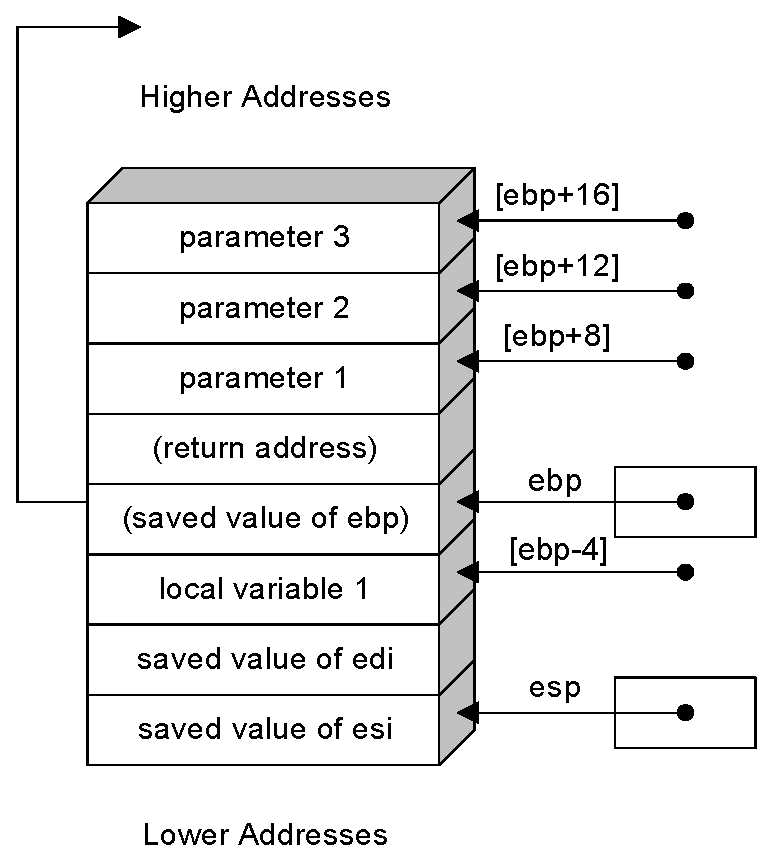
\includegraphics[width=4in]{x86-32bit/x86-activation-record.pdf}
\caption{A picture of the stack in memory during the execution of the body of myFunc}
\label{x86-activation-record.fig}
\end{figure}

The assembly code for {\tt myFunc()} was shown above in
Listing~\ref{x86-callee-example-1.s.lst}. The C++ code to call that
subroutine is shown in
Listing~\ref{x86-callee-example-main.cpp.lst}.

\begin{figure}[h!]
\lstinputlisting[caption={Example C++ code to invoke a 3-parameter x86 subroutine},label={x86-callee-example-main.cpp.lst},backgroundcolor=\color{white},frame=trBL,linewidth=6.9in,xleftmargin=0.15in,language=C++]{x86-32bit/code/callee-example-main.cpp}
\end{figure}







\chapter{64-bit x86 Assembly}

\begin{quotation}
\ldots
\end{quotation}

\noindent {\em This chapter was derived from a document written by Adam Ferrari and later updated by Alan Batson, Mike Lack, Anita
Jones, and Aaron Bloomfield}

\section{Introduction}

This small guide, in combination with the material covered in the
class lectures on assembly language programming, should provide enough
information to do the assembly language labs for this class. In this
guide, we describe the basics of 64-bit x86 assembly language
programming, covering a small but useful subset of the available
instructions and assembler directives. However, real x86 programming
is a large and extremely complex universe, much of which is beyond the
useful scope of this class. For example, there exists real (albeit
older) x86 code running in the world was written using the 16-bit
subset of the x86 instruction set. Using the 16-bit programming model
can be quite complex~-- it has a segmented memory model, more
restrictions on register usage, and so on. This was expanded into a
32-bit programming model in 1985, but that had the limit of only 4 Gb
of memory.  In this guide we'll restrict our attention to the more
modern aspects of 64-bit x86 programming, and delve into the
instruction set only in enough detail to get a basic feel for
programming x86 compatible chips at the hardware level.

\section{Registers}

Modern 64-bit x86 processors have sixteen 64-bit general purpose
registers, as depicted in Figure~\ref{x86-register-diagram.fig}. The
register names for the first eight registers are mostly historical in
nature; the last eight registers were given sequential numbers. For
example, RAX used to be EAX (in the 32-bit machine), which used to be
called the ``accumulator'' since it was used by a number of arithmetic
operations, and RCX (32-bit version: ECX) was known as the ``counter''
since it was used to hold a loop index. Whereas most of the registers
have lost their special purposes in the modern instruction set, by
convention, two are sometimes reserved for special purposes~-- the
stack pointer (RSP) and the base pointer (RBP).

\begin{figure}[h]
\begin{center}
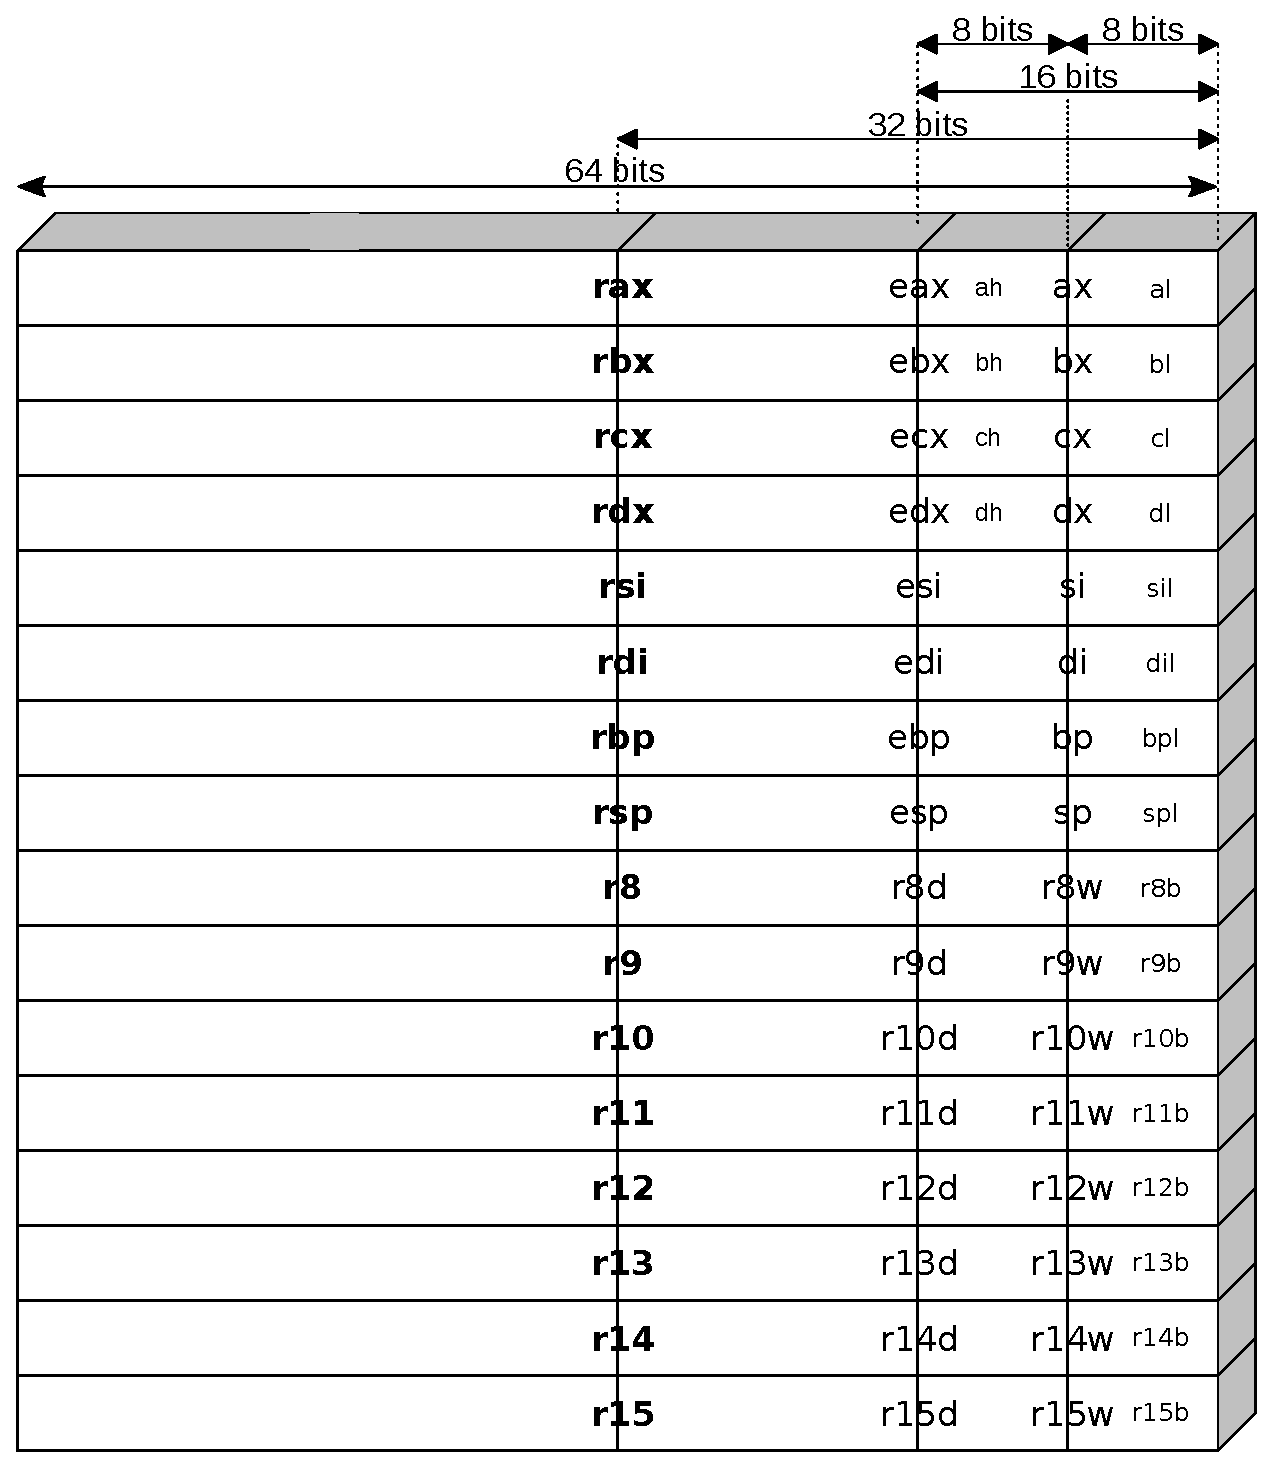
\includegraphics[width=4in]{x86-64bit/x86-register-diagram.pdf}
\end{center}
\caption{The x86 register set}
\label{x86-register-diagram.fig}
\end{figure}

In all cases, subsections of the registers may be used.  For example,
the least significant 2 bytes of RAX can be treated as a 16-bit
register called AX.  The least significant byte of AX can be used as a
single 8-bit register called AL, while the most significant byte of AX
can be used as a single 8-bit register called AH. It is important to
realize that these names refer to the same physical register. When a
two-byte quantity is placed into DX, the update affects the value of
RDX (in particular, the least significant 16 bits of RDX). These
``sub-registers'' are mainly hold-overs from older, 16-bit versions of
the instruction set. However, they are sometimes convenient when
dealing with data that are smaller than 64-bits (e.g., 1-byte ASCII
characters).  Note that four of the registers (EAX, EBX, ECX, and EDX)
have an addition ``sub-register'' spot: the second to last byte of the
register.

When referring to registers in assembly language, the names are not
case-sensitive. For example, the names RAX and rax refer to the same
register.

\section{Memory and Addressing Modes}

\subsection{Declaring Static Data Regions}

You can declare static data regions (analogous to global variables) in
x86 assembly using special assembler directives for this purpose.
Data declarations should be preceded by the .DATA directive. Following
this directive, the directives DB, DW, and DD can be used to declare
one, two, and four byte data locations, respectively. Declared
locations can be labeled with names for later reference - this is
similar to declaring variables by name, but abides by some lower level
rules. For example, locations declared in sequence will be located in
memory next to one another.  Some example declarations are depicted in
Listing~\ref{x86-declaring-memory-regions.lst}.

\begin{figure}[h]
\lstinputlisting[caption=Declaring x86 memory regions,label={x86-declaring-memory-regions.lst},backgroundcolor=\color{white},frame=trBL,linewidth=7in,xleftmargin=0in,language={[x86masm]Assembler}]{x86-64bit/code/memory-regions.s}
\end{figure}

The last example in Listing~\ref{x86-declaring-memory-regions.lst}
illustrates the declaration of an array.  Unlike in high level
languages where arrays can have many dimensions and are accessed by
indices, arrays in assembly language are simply a number of cells
located contiguously in memory. Two other common methods used for
declaring arrays of data are the TIMES directive and the use of string
literals. The TIMES directive tells the assembler to duplicate an
expression a given number of times. For example, the statement ``TIMES
4 DB 2'' is equivalent to ``2, 2, 2, 2''. Some examples of declaring
arrays are depicted in Listing~\ref{x86-declaring-arrays.lst}.

\begin{figure}[h]
\lstinputlisting[caption=Declaring x86 arrays in memory,label={x86-declaring-arrays.lst},backgroundcolor=\color{white},frame=trBL,linewidth=7in,xleftmargin=0in,language={[x86masm]Assembler}]{x86-64bit/code/declaring-arrays.s}
\end{figure}

\subsection{Addressing Memory}
\label{addressing-memory.sec}

Modern x86-compatible processors are capable of addressing up to
$2^{64}$ bytes of memory; that is, memory addresses are 64-bits wide.
For example, in Listings~\ref{x86-declaring-memory-regions.lst} and
\ref{x86-declaring-arrays.lst}, where we used labels to refer to memory
regions, these labels are actually replaced by the assembler with
64-bit quantities that specify addresses in memory. In addition to
supporting referring to memory regions by labels (i.e. constant
values), the x86 provides a flexible scheme for computing and
referring to memory addresses:

{\bf x86 Addressing Mode Rule}~-- Up to two of the 64-bit registers
and a 64-bit signed constant can be added together to compute a memory
address. One of the registers can be optionally pre-multiplied by 2,
4, or 8.

To see this memory addressing rule in action, we'll look at some
example mov instructions.  As we'll see later in
Section~\ref{data-movement-instructions.sec}, the {\tt mov} instruction
moves data between registers and memory.  This instruction has two
operands~-- the first is the destination (where we're moving data {\em
  to}) and the second specifies the source (where we're getting the
data {\em from}). Some examples of mov instructions using address
computations that obey the above rule are shown in
Listing~\ref{x86-valid-addressing-modes.lst}.

\begin{figure}[h]
\lstinputlisting[caption={Valid x86 addressing modes},label={x86-valid-addressing-modes.lst},backgroundcolor=\color{white},frame=trBL,linewidth=7in,xleftmargin=0in,language={[x86masm]Assembler}]{x86-64bit/code/valid-addressing-modes.s}
\end{figure}

Some examples of incorrect address calculations are shown in Listing~\ref{x86-invalid-addressing-modes.lst}.

\begin{figure}[h]
\lstinputlisting[caption={Invalid x86 addressing modes},label={x86-invalid-addressing-modes.lst},backgroundcolor=\color{white},frame=trBL,linewidth=7in,xleftmargin=0in,language={[x86masm]Assembler}]{x86-64bit/code/invalid-addressing-modes.s}
\end{figure}


\subsection{Size Directives}

In general, the intended size of the of the data item at a given
memory address can be inferred from the assembly code instruction in
which it is referenced. For example, in all of the above instructions,
the size of the memory regions could be inferred from the size of the
register operand~-- when we were loading a 64-bit register, the
assembler could infer that the region of memory we were referring to
was 8 bytes wide. When we were storing the value of a one byte
register to memory, the assembler could infer that we wanted the
address to refer to a single byte in memory.  However, in some cases
the size of a referred-to memory region is ambiguous. Consider the
instruction {\tt mov [ebx], 2}.


Should this instruction move the value 2 into the single byte at
address EBX? Perhaps it should move the 64-bit integer representation
of 2 into the 4-bytes starting at address EBX. Since either is a valid
possible interpretation, the assembler must be explicitly directed as
to which is correct.  The size directives {\tt BYTE PTR}, {\tt WORD
  PTR}, {\tt DWORD PTR}, and {\tt QWORD PTR} serve this purpose. For
examples, see Listing~\ref{x86-size-directives.lst}.

\begin{figure}[h]
\lstinputlisting[caption={x86 size directive usage},label={x86-size-directives.lst},backgroundcolor=\color{white},frame=trBL,linewidth=7in,xleftmargin=0in,language={[x86masm]Assembler}]{x86-64bit/code/size-directives.s}
\end{figure}


\section{Instructions}

Machine instructions generally fall into three categories: data movement, arithmetic/logic,
and control-flow. In this section, we will look at important examples of x86 instructions from
each category. This section should not be considered an exhaustive list of x86 instructions, but
rather a useful subset.

In this section, we will use the following notation:

\begin{itemlist}
\item $<$reg64$>$ - means any 64-bit register described in Section 2, for example, ESI.
\item $<$reg16$>$ - means any 16-bit register described in Section 2, for example, BX.
\item $<$reg32$>$ - means any 32-bit register described in Section 2, for example, BX.
\item $<$reg8$>$ - means any 8-bit register described in Section 2, for example AL.
\item $<$reg$>$ - means any of the above.
\item $<$mem$>$ - will refer to a memory address, as described in Section~\ref{addressing-memory.sec}, for example {\tt [EAX]}, or
{\tt [var+4]}, or {\tt DWORD PTR [RAX+RBX]}.
\item $<$con64$>$ - means any 64-bit constant.
\item $<$con32$>$ - means any 32-bit constant.
\item $<$con16$>$ - means any 16-bit constant.
\item $<$con8$>$ - means any 8-bit constant.
\item $<$con$>$ - means any of the above sized constants.
\end{itemlist}

\subsection{Data Movement Instructions}
\label{data-movement-instructions.sec}

\asminstructionsummary{mov}
{mov $<$reg$>$,$<$reg$>$\newline mov $<$reg$>$,$<$mem$>$\newline mov $<$mem$>$,$<$reg$>$\newline mov $<$reg$>$,$<$const$>$\newline mov $<$mem$>$,$<$const$>$}
{The mov instruction moves the data item referred to by its second
  operand (i.e.  register contents, memory contents, or a constant
  value) into the location referred to by its first operand (i.e. a
  register or memory). While register-to-register moves are possible,
  direct memory-to-memory moves are not. In cases where memory
  transfers are desired, the source memory contents must first be
  loaded into a register, then can be stored to the destination memory
  address.}
{mov rax, rbx \linebreak mov BYTE PTR [var], 5 }
{; transfer ebx to eax\linebreak; store the value 5 into the byte at\linebreak; memory location ``var''}
{2.2in}{3.5in}

\asminstructionsummary{push}
{push $<$reg$>$\newline push $<$mem$>$\newline push $<$con64$>$}
{The push instruction places its operand onto the top of the hardware supported
stack in memory. Specifically, push first decrements RSP by 8, then places its
operand into the contents of the 64-bit location at address [RSP]. RSP (the stack
pointer) is decremented by push since the x86 stack grows down~-- i.e. the stack
grows from high addresses to lower addresses.}
{push rax\newline push [var]}
{; push the contents of rax onto the stack\newline
; push the 8 bytes at address ``var'' onto stack}
{1in}{4.7in}

\asminstructionsummary{pop}
{pop $<$reg$>$\newline pop $<$mem$>$}
{The pop instruction removes the 8-byte data element from the top of
  the hardware supported stack into the specified operand (i.e.
  register or memory location). Specifically, pop first moves the 8
  bytes located at memory location [RSP] into the specified register or
  memory location, and then increments SP by 8.}
{pop rdi \newline pop [rbx]}
{; pop the top element of the stack into RDI.\newline
; pop the top element of the stack into memory at\newline
; the four bytes starting at location RBX.}
{1in}{4.7in}

\asminstructionsummary{lea}
{lea $<$reg64$>$,$<$mem$>$}
{The lea instruction places the address specified by its second
  operand into the register specified by its first operand. Note, the
  contents of the memory location are not loaded~-- only the effective
  address is computed and placed into the register.  This is useful
  for obtaining a ``pointer'' into a memory region.}
{lea rax, [var]\newline lea rdi, [rbx+4*rsi]}
{; the address of ``var'' is placed in RAX \newline
; the value RBX+4*RSI is placed in RDI}
{1.85in}{3.85in}

\subsection{Arithmetic and Logic Instructions}

\asminstructionsummary{add, sub}
{add $<$reg$>$,$<$reg$>$ \hspace{0.5in} sub $<$reg$>$,$<$reg$>$ \newline
add $<$reg$>$,$<$mem$>$ \hspace{0.5in} sub $<$reg$>$,$<$mem$>$ \newline
add $<$mem$>$,$<$reg$>$ \hspace{0.5in} sub $<$mem$>$,$<$reg$>$ \newline
add $<$reg$>$,$<$con$>$ \hspace{0.5in} sub $<$reg$>$,$<$con$>$ \newline
add $<$mem$>$,$<$con$>$ \hspace{0.5in} sub $<$mem$>$,$<$con$>$}
{The add instruction adds together its two operands, storing the
  result in its first operand. Similarly, the sub instruction
  subtracts its second operand from its first.  Note, whereas both
  operands may be registers, at most one operand may be a memory
  location.}
{add rax, 10\newline 
sub [var], rsi\newline\newline\newline
add BYTE PTR [var], 10}
{; add 10 to the contents of RAX. \newline
; subtract the contents of RSI from \newline
; the 64-bit integer stored at \newline
; memory location ``var''.\newline
; add 10 to the single byte stored\newline
; at memory address ``var''.\newline}
{2.2in}{3.5in}

\asminstructionsummary{inc, dec}
{inc $<$reg$>$ \hspace{0.5in} dec $<$reg$>$\newline
inc $<$mem$>$ \hspace{0.5in} dec $<$mem$>$}
{The inc instruction increments the contents of its operand by one,
  and similarly dec decrements the contents of its operand by one.}
{dec rax \newline inc DWORD PTR [var]}
{; subtract one from the contents of RAX. \newline
; add one to the 64-bit integer stored at \newline
; memory location ``var''.}
{1.8in}{3.9in}

\asminstructionsummary{imul}
{imul $<$reg64$>$,$<$reg64$>$\newline
imul $<$reg64$>$,$<$mem$>$\newline
imul $<$reg64$>$,$<$reg64$>$,$<$con$>$\newline
imul $<$reg64$>$,$<$mem$>$,$<$con$>$}
{The imul instruction has two basic formats: two-operand (first two
syntax listings above) and three-operand (last two syntax listings
above).  The two-operand form multiplies its two operands together and
stores the result in the first operand. The result (i.e., first)
operand must be a register.  The three operand form multiplies its
second and third operands together and stores the result in its first
operand. Again, the result operand must be a register.  Furthermore,
the third operand is restricted to being a constant value.}
{imul rax, [var]\newline\newline\newline
imul rsi, rdi, 25}
{; multiply the contents of RAX by the \newline
; 64-bit contents of the memory location \newline
; ``var''. Store the result in RAX.\newline
; multiply the contents of RDI by 25. \newline
; Store the result in RSI.}
{1.8in}{3.9in}

\asminstructionsummary{idiv}
{idiv $<$reg64$>$\newline
idiv $<$mem$>$}
{The idiv instruction is used to divide the contents of the 64 bit
  integer RDX:RAX (constructed by viewing RDX as the most significant
  eight bytes and RAX as the least significant eight bytes) by the
  specified operand value. The quotient result of the division is
  stored into RAX, while the remainder is placed in RDX. This
  instruction must be used with care. Before executing the
  instruction, the appropriate value to be divided must be placed into
  RDX and RAX. Clearly, this value is overwritten when the idiv
  instruction is executed.}
{idiv rbx \newline\newline\newline idiv DWORD PTR [var]}
{; divide the contents of RDX:RAX by the \newline
; contents of RBX. Place the quotient \newline
; in RAX and the remainder in RDX.\newline
; same as above, but divide by the \newline
; 64-bit value stored at memory \newline
; location ``var''.}
{1.9in}{3.8in}

\asminstructionsummary{and, or, xor}
{and $<$reg$>$,$<$reg$>$ \hspace{0.25in} or $<$reg$>$,$<$reg$>$ \hspace{0.25in} xor $<$reg$>$,$<$reg$>$ \newline
and $<$reg$>$,$<$mem$>$ \hspace{0.25in} or $<$reg$>$,$<$mem$>$ \hspace{0.25in} xor $<$reg$>$,$<$mem$>$ \newline
and $<$mem$>$,$<$reg$>$ \hspace{0.25in} or $<$mem$>$,$<$reg$>$ \hspace{0.25in} xor $<$mem$>$,$<$reg$>$ \newline
and $<$reg$>$,$<$con$>$ \hspace{0.25in} or $<$reg$>$,$<$con$>$ \hspace{0.25in} xor $<$reg$>$,$<$con$>$ \newline
and $<$mem$>$,$<$con$>$ \hspace{0.25in} or $<$mem$>$,$<$con$>$ \hspace{0.25in} xor $<$mem$>$,$<$con$>$}
{These instructions perform the specified logical operation (logical
bitwise and, or, and exclusive or, respectively) on their operands,
placing the result in the first operand location.}
{and rax, 0fH \newline xor rdx, rdx}
{; clear all but the last 4 bits of RAX. \newline ; set the contents of RDX to zero.}
{1.7in}{4in}

\asminstructionsummary{not}
{not $<$reg$>$ \newline not $<$mem$>$}
{Performs the logical negation of the operand contents (i.e., flips all bit values).}
{not BYTE PTR [var]}
{; negate all bits in the byte at the \newline ; memory location ``var''.}
{1.7in}{4in}

\asminstructionsummary{neg}
{neg $<$reg$>$ \newline neg $<$mem$>$}
{Performs the arithmetic (i.e., two's complement) negation of the operand contents.}
{neg rax \newline neg [var]}
{; negate the contents of RAX. \newline ; negate the contests of ``var''}
{1.4in}{4.3in}

\asminstructionsummary{shl, shr}
{shl $<$reg$>$,$<$con8$>$ \hspace{0.5in} shr $<$reg$>$,$<$con8$>$\newline
shl $<$mem$>$,$<$con8$>$ \hspace{0.5in} shr $<$mem$>$,$<$con8$>$\newline
shl $<$reg$>$,cl \hspace{0.92in} shr $<$reg$>$,cl\newline
shl $<$mem$>$,cl \hspace{0.92in} shr $<$mem$>$,cl}
{These instructions shift the bits in their first operand's contents
  left and right ({\tt shl} and {\tt shr}, respectively), padding the
  resulting empty bit positions with zeros. The shifted operand can be
  shifted up to 31 places. The number of bits to shift is specified
  by the second operand, which can be either an 8-bit constant or the
  register CL. In either case, shifts counts of greater then 31 are
  performed modulo 64.}
{shl rax 5 \newline\newline shr [var] 3}{; shift the contents of rax left by 5 bit \newline ; positions \newline ; shift the contents of ``var'' right by 3 \newline ; bit positions}{1.4in}{4.3in}

\subsection{Control Flow Instructions}

In this section, we will refer to labeled locations in the program
text as $<$label$>$. Labels can be inserted anywhere in x86 assembly
code text by entering a label name followed by a colon. For example,
consider the code fragment in Listing~\ref{x86-labeled-code-location.lst}.
The second instruction in this code fragment is labeled ``begin''.
Elsewhere in the code, we can refer to the memory location that this
instruction is located at in memory using the more convenient symbolic
name ``begin'' instead of having to refer to the memory address as an
integer.

\begin{figure}[h]
\lstinputlisting[caption={x86 labeled code location},label={x86-labeled-code-location.lst},backgroundcolor=\color{white},frame=trBL,linewidth=4.75in,xleftmargin=2.25in,language={[x86masm]Assembler}]{x86-64bit/code/labeled-code-location.s}
\end{figure}


\asminstructionsummary{jmp}
{jmp $<$label$>$}
{Transfers program control flow to the instruction at the memory
  location indicated by the operand.}
{jmp begin}{; jumps to the ``begin'' label}
{1.5in}{3.7in}

\asminstructionsummary{jCC}
{je $<$label$>$ ; Jump when equal\newline
jne $<$label$>$ ; Jump when not equal\newline
jz $<$label$>$ ; Jump when last result was zero\newline
jg $<$label$>$ ; Jump when greater than\newline
jge $<$label$>$ ; Jump when greater than or equal to\newline
jl $<$label$>$ ; Jump when less than\newline
jle $<$label$>$ ; Jump when less than or equal to}
{These instructions are conditional jumps that are based on the status
  of a set of {\bf condition codes} that are stored in a special
  register called the {\em machine status word}. The contents of the
  machine status word include information about the last arithmetic
  operation performed. For example, one bit of this word indicates if
  the last result was zero. Another indicates if the last result was
  negative.  Based on these condition codes, a number of conditional
  jumps can be performed. For example, the jz instruction performs a
  jump to the specified operand label if the result of the last
  arithmetic operation (e.g. add, sub, etc.) was zero. Otherwise,
  control proceeds to the next instruction in sequence after the jz.
  These conditional jumps are the underlying support needed to
  implement high-level language features such as ``if'' statements and
  loops (e.g. ``while'' and ``for''). \vspace{6pt}\newline
  A number of the conditional branches are given names that are
  intuitively based on the last operation performed being a special
  compare instruction, cmp (see below).  For example, conditional
  branches such as jle and jne are based on first performing a cmp
  operation on the desired operands.}
{cmp rax, rbx \newline jle done}
{; if the contents of rax are less than or \newline
; equal to the contents of ebx, jump to the \newline
; code location labeled ``done''.}
{1.4in}{4.3in}

\asminstructionsummary{cmp}
{cmp $<$reg$>$,$<$reg$>$\newline
cmp $<$reg$>$,$<$mem$>$\newline
cmp $<$mem$>$,$<$reg$>$\newline
cmp $<$reg$>$,$<$con$>$\newline
cmp $<$mem$>$,$<$con$>$}
{Compares the two specified operands, setting the condition codes in
  the machine status word appropriately. In fact, this instruction is
  equivalent to the sub instruction, except the result of the
  subtraction is discarded.}
{cmp DWORD PTR [var], 10\newline jeq loop}
{; if the 4 bytes stored at memory\newline
; location ``var'' equal the 4-byte\newline
;  integer value 10, then jump to the\newline
; code location labeled loop}
{2.2in}{3.5in}

\asminstructionsummary{call}
{call $<$label$>$}
{This instruction implements a subroutine call that operates in
cooperation with the subroutine return instruction, ret, described
below. This instruction first pushes the current code location onto
the hardware supported stack in memory (see the push instruction for
details), and then performs an unconditional jump to the code location
indicated by the label operand. The added value of this instruction
(as compared to the simple jmp instruction) is that it saves the
location to return to when the subroutine completes.}
{call my\_subroutine}
{; jumps to the ``my\_subroutine'' label, \newline
; pushing the return address onto the \newline
; stack}
{1.8in}{3.9in}

\asminstructionsummary{ret}
{ret}
{In cooperation with the call instruction, the ret instruction
  implements a subroutine return mechanism. This instruction first
  pops a code location off the hardware supported in-memory stack (see
  the pop instruction for details). It then performs an unconditional
  jump to the retrieved code location.}
{ret}{; returns to the address on the top of the stack}
{1in}{4.7in}


\section{Basic Program Structure}
\label{x86-basic-program-structure.sec}

\begin{wrapfigure}{r}{0.37\textwidth}
\lstinputlisting[backgroundcolor=\color{white},frame=trBL,linewidth=2.5in,xleftmargin=0.25in,label={x86-return2.s.lst},language={[x86masm]Assembler},caption={x86 code to return 2}]{x86-64bit/code/return2.s}
\vspace{-0.25in}
\end{wrapfigure}

Given the above repertoire of instructions, you are in a position to
examine the basic skeletal structure of an assembly language
subroutine suitable for linking into C++ code. Unlike C++, which is
often used for the development of complete software systems, assembly
language is most often used in cooperation with other languages such
as Fortran, C, and C++. Commonly, most of a project is implemented in
the more convenient high-level language, and assembly language is used
sparingly to implement extremely low-level hardware interfaces or
performance-critical ``inner loops.'' Thus, in addition to
understanding how to program in assembly language, it is equally
important to understand how to link assembly language code into
high-level language programs.

Before examining the linkage conventions, we must first examine the
basic structure of an assembly language file. To do this, we can
compare a very simple assembly language file to an equivalent C++
file. In Listings~\ref{x86-return2.s.lst} and \ref{x86-return2.cpp.lst} we see
two files, one in C++, the other in x86 assembly. Each file includes a
function (albeit an ugly one) to return the integer value 2.

Note that the fucntion shown in assembly in
Listing~\ref{x86-return2.s.lst} returns a 32-bit value, since it is
put into register eax.  This corresponds to retnring an {\tt int} in C
or C++.  If we wanted to return a 64-bit value, which corresponds to
returning a {\tt long}, then we would put the return value into rax.

The top of the assembly file contains two directives that indicate the
instruction set and memory model we will use for all work in this
class (note, there are other possibilities~-- one might use only the
older 80286 instruction set for wider compatibility, for example).

Next, where in the C++ file we find the declaration of the global
variable ``var'', in the assembly file we find the use of the .DATA
and DD directives (described in Section 3.1) to reserve and initialize
a 4-byte (i.e., integer-sized) memory region labeled ``var''.

\begin{wrapfigure}{r}{0.37\textwidth}
\lstinputlisting[backgroundcolor=\color{white},frame=trBL,linewidth=2.5in,xleftmargin=0.25in,label={x86-return2.cpp.lst},language=C++,caption={C++ code to return 2}]{x86-64bit/code/return2.cpp}
\vspace{-0.25in}\end{wrapfigure}

Next in each file, we find the declaration of the function named
returnTwo. In the C++ file we have declared the function to be extern
``C''. This declaration indicates that the C++ compiler should use C
naming conventions when labeling the function returnTwo in the
resulting object file that it produces. In fact, this naming
convention means that the function returnTwo should map to the label
\_returnTwo in the object code. In the assembly code, we have labeled
the beginning of the subroutine \_returnTwo using the PROC directive,
and have declared the label \_returnTwo to be public. Again, the
result of these actions will be that the subroutine will map to the
symbol \_returnTwo in the object code that the assembler generates.

The function bodies are straight-forward. As we will see in more
detail in Section 6, return values for functions are placed into EAX
by convention, hence the instruction to move the contents of ``var''
into EAX in the assembly code.

\begin{wrapfigure}{r}{0.48\textwidth}
\lstinputlisting[backgroundcolor=\color{white},frame=trBL,linewidth=4in,xleftmargin=0.25in,label={x86-calling-return2.cpp.lst},language=C++,caption={Calling returnTwo() from C++}]{x86-64bit/code/calling-return2.cpp}
\vspace{-0.25in}
\end{wrapfigure}

Given these equivalent function definitions, use of either version of
the function is the same.  A sample call to the function returnTwo is
depicted in Listing~\ref{x86-calling-return2.cpp.lst}. This C++ code
could be linked to either definition of the function and would produce
the same results (note, we could not link to both definitions, or the
linker would produce a ``multiply defined symbol'' error. The
mechanics of program linking will be discussed in an associated
document that relates to the specific programming environment that you
will use to assemble and run programs.


\chapter{The 64-bit x86 C Calling Convention}

\begin{quotation}
\ldots
\end{quotation}

\noindent {\em This chapter was derived from a document written by Adam Ferrari and later updated by Alan Batson, Mike Lack, Anita
Jones, and Aaron Bloomfield}

\section{What is a Calling Convention?}

At the end of the previous chapter, we saw a simple example of a
subroutine defined in x86 assembly language. In fact, this subroutine
was quite simple~-- it did not modify any registers except EAX (or
RAX) (which was needed to return the result), and it did not call any
other subroutines. In practice, such simple function definitions are
rarely useful. When more complex subroutines are combined in a single
program, a number of complicating issues arise.  For example, how are
parameters passed to a subroutine? Can subroutines overwrite the
values in a register, or does the caller expect the register contents
to be preserved? Where should local variables in a subroutine be
stored? How should results be returned from functions?

To allow separate programmers to share code and develop libraries for
use by many programs, and to simplify the use of subroutines in
general, programmers typically adopt a common {\em calling
  convention}. The calling convention is simply a set of rules that
answers the above questions without ambiguity to simplify the
definition and use of subroutines. For example, given a set of calling
convention rules, a programmer need not examine the definition of a
subroutine to determine how parameters should be passed to that
subroutine. Furthermore, given a set of calling convention rules,
high-level language compilers can be made to follow the rules, thus
allowing hand-coded assembly language routines and high-level language
routines to call one another.

In practice, even for a single processor instruction set, many calling
conventions are possible.  In this class we will examine and use one
of the most important conventions: the C language calling convention.
Understanding this convention will allow you to write assembly
language subroutines that are safely callable from C and C++ code, and
will also enable you to call C library functions from your assembly
language code.

\section{The C Calling Convention}

The C calling convention is based heavily on the use of the
hardware-supported stack. To understand the C calling convention, you
should first make sure that you fully understand the push, pop, call,
and ret instructions~-- these will be the basis for most of the rules.
In this calling convention, subroutine parameters are passed on the
stack. Registers are saved on the stack, and local variables used by
subroutines are placed in memory on the stack. In fact, this
stack-centric implementation of subroutines is not unique to the C
language or the x86 architecture. The vast majority of high-level
procedural languages implemented on most processors have used similar
calling convention.

The calling convention is broken into two sets of rules. The first set
of rules is employed by the caller of the subroutine, and the second
set of rules is observed by the writer of the subroutine (the
``callee''). It should be emphasized that mistakes in the observance
of these rules quickly result in fatal program errors; thus meticulous
care should be used when implementing the call convention in your own
subroutines.

\section{The Caller's Rules}

The caller should adhere to the following rules when invoking a
subroutine:

\begin{numlist}
\item Before calling a subroutine, the caller should save the contents
  of certain registers that are designated caller-saved. The
  caller-saved registers are r10, r11, and any registers that
  parameters are put into. If you want the contents of these registers
  to be preserved across the subroutine call, push them onto the
  stack.
\item To pass parameters to the subroutine, we put up to six of them
  into registers (in order: rdi, rsi, rdx, rcx, r8, r9).  If there are
  more than six parameters to the subroutine, then push the rest onto
  the stack in {\em reverse order} (i.e. last parameter first)~--
  since the stack grows down, the first of the extra parameters
  (really the seventh parameter) parameter will be stored at the
  lowest address (this inversion of parameters was historically used
  to allow functions to be passed a variable number of parameters).
\item To call the subroutine, use the {\tt call} instruction. This
  instruction places the return address on top of the parameters on
  the stack, and branches to the subroutine code.
\item After the subroutine returns, (i.e. immediately following the
  call instruction) the caller must remove any additional parameters
  (beyond the six stored in registers) from stack.  This restores the
  stack to its state before the call was performed.
\item The caller can expect to find the return value of the subroutine
  in the register RAX.
\item The caller restores the contents of caller-saved registers (r10,
  r11, and any in the parameter passing registers) by popping them off
  of the stack. The caller can assume that no other registers were
  modified by the subroutine.
\end{numlist}

Due to the way the calling convention is structured, it will typically
be the case that some (or most) of these steps will not make any
changes to the stackd.  For example, if there are six or fewer
parameters, then nothing is pushed onto the stack in that step.
Likewise, programmers (and compilers) tyipcally keep the results they
care about out of the caller-saved registers in steps 1 and 6 to
prevent excess pushes and pops.

\section{The Callee's Rules}

The definition of the subroutine should adhere to the following rules:

\begin{numlist}

\item Allocate local variables by using registers or making space on
  the stack.  Recall, the stack grows down, so to make space on the
  top of the stack, the stack pointer should be decremented. The
  amount by which the stack pointer is decremented depends on the
  number of local variables needed. For example, if a local {\tt
    float} and a local {\tt long} (12 bytes total) were required, the
  stack pointer would need to be decremented by 12 to make space for
  these local variables:

\begin{lstlisting}[backgroundcolor=\color{white},frame=trBL,linewidth=3.75in,xleftmargin=2.25in,label={x86-callee-code-2.lst},language={[x86masm]Assembler},caption={x86 callee code, part 2}]
sub rsp, 12
\end{lstlisting}

As with parameters, local variables will be located at known offsets
from the stack pointer.

\item Next, the values of any registers that are designated
  callee-saved that will be used by the function must be saved. To
  save registers, push them onto the stack. The callee-saved registers
  are RBX, RBP, and R12 through R15 (RSP will also be preserved by the
  call convention, but need not be pushed on the stack during this
  step).

  After these three actions are performed, the actual operation of the
  subroutine may proceed.  When the subroutine is ready to return, the
  call convention rules continue:

\item When the function is done, the return value for the function
  should be placed in RAX if it is not already there.

\item The function must restore the old values of any callee-saved
  registers (RBX, RBP, and R12 through R15) that were modified. The
  register contents are restored by popping them from the stack. Note,
  the registers should be popped in the inverse order that they were
  pushed.

\item Next, we deallocate local variables. The easiest way to do this
  is to add to RSP the same amount that was subtracted from it in step
  1.

\item Finally, we return to the caller by executing a {\tt ret}
  instruction. This instruction will find and remove the appropriate
  return address from the stack.

\end{numlist}

If you look at the assembly generated by some compilers, you will see
a few extra commands in there in the callee's prologue:

\begin{lstlisting}[backgroundcolor=\color{white},frame=trBL,linewidth=5.5in,xleftmargin=1.25in,label={x86-callee-code-2.lst},language={[x86masm]Assembler},caption={x86 extraneous codedd}]
push rbp       ; at the start of the callee
mov rbp, rsp
...
pop rbp        ; just before the ending 'ret'
\end{lstlisting}

This code is unnecessary, and is a hold-over from the 32-bit calling
convention.  You can tell the compiler to not include this code by
invoking it with the {\tt -fomit-frame-pointer} flag.

It might be noted that the callee's rules fall cleanly into two halves
that are basically mirror images of one another. The first half of the
rules apply to the beginning of the function, and are therefor
commonly said to define the {\em prologue} to the function. The latter
half of the rules apply to the end of the function, and are thus
commonly said to define the {\em epilogue} of the function.

\section{Calling Convention Example}

The above rules may seem somewhat abstract on first examination. In practice, the rules
become simple to use when they are well understood and familiar. To start the process of better
understanding the call convention, we now examine a simple example of a subroutine call and a
subroutine definition.

\begin{figure}[h!]
\lstinputlisting[caption={Example function call, caller's rules obeyed},label={x86-caller-example-1.s.lst},backgroundcolor=\color{white},frame=trBL,linewidth=6in,xleftmargin=0.75in,language={[x86masm]Assembler}]{x86-64bit/code/caller-example-1.s}
\end{figure}


In Listing~\ref{x86-caller-example-1.s.lst} a sample function call is
depicted. The three parameters are put into the parameter passing
registers; if there were more than 6, then the additional ones would
be pushed onto the stack in reverse order.  The call instruction is
used to jump to the beginning of the subroutine in anticipation of the
fact that the subroutine will use the ret instruction to return when
the subroutine completes. When the subroutine returns, the parameters
must be removed from the stack. A simple way to do this is to add the
appropriate amount to the stack pointer (since the stack grows down).
Finally, the result is available in RAX.

Next up is the caller's rules. An example subroutine implementation
that obeys the callee's rules is depicted in
Listing~\ref{x86-callee-example-1.s.lst}. The subroutine prologue
performs the standard actions of allocating local variables by
decrementing the stack pointer, and saving register values on the
stack.

\begin{figure}[h!]
\lstinputlisting[caption={Example function definition, callee's rules obeyed},label={x86-callee-example-1.s.lst},backgroundcolor=\color{white},frame=trBL,linewidth=6.9in,xleftmargin=0.15in,language={[x86masm]Assembler}]{x86-64bit/code/callee-example-1.s}
\end{figure}

In the body of the subroutine we can how the local variables are
accessed.  The prologue put 24 bytes of ``stuff'' onto the stack:
three 8 byte values.  The first was the local variable (via the {\tt
  sub rsp, 8} call).  The second was the rbx backup, and the third was
the rbp backup.  Thus, the stack pointer is now 16 bytes below the
local variable, as two 8 byte ``things'' have been pushed onto the
stack since the local variable was allocated.  Thus, to access the
local variable, one uses {\tt [rsp+16]}, as seen throughout the code.

The function epilogue, as expected, is basically a mirror image of the
function prologue. The caller's register values are recovered from the
stack, the local variables are deallocated by resetting the stack
pointer, and the {\tt ret} instruction is used to return to the
appropriate code location in the caller.

A good way to visualize the operation of the calling convention is to
draw the contents of the nearby region of the stack during subroutine
execution. Figure~\ref{x86-activation-record.fig} depicts the contents
of the stack during the execution of the body of myFunc (myFunc is
depicted in Listing~\ref{x86-callee-example-1.s.lst}). Notice, lower
addresses are depicted lower in the figure, and thus the ``top'' of
the stack is the bottom-most cell. This corresponds visually to the
intuitive statement that the x86 hardware stack ``grows down.'' The
cells depicted in the stack are 64-bit wide memory locations, thus the
memory addresses of the cells are 4 bytes apart. From this picture we
see clearly why the first parameter resides at an offset of 8 bytes
from the base pointer. Above the parameters on the stack (and below
the base pointer), the call instruction placed the return address,
thus leading to an extra 4 bytes of offset from the base pointer to
the first parameter.

\begin{figure}[h]
\centering
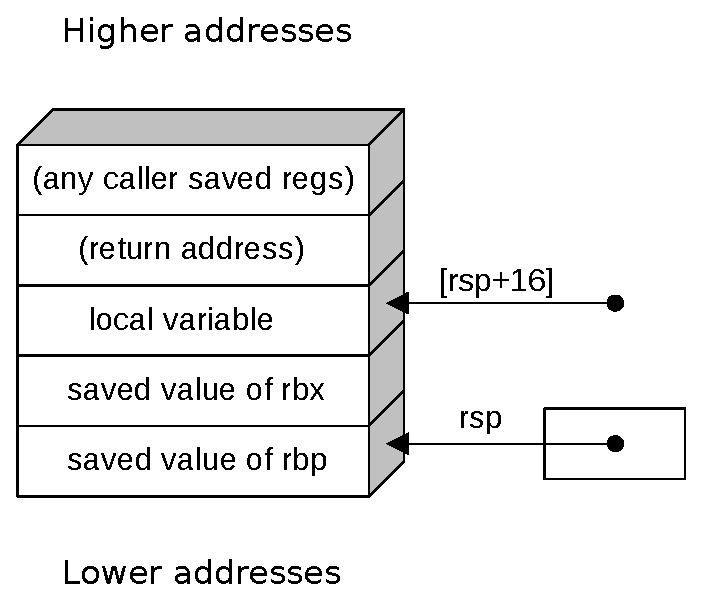
\includegraphics[width=4in]{x86-64bit/x86-activation-record.pdf}
\caption{A picture of the stack in memory during the execution of the body of myFunc}
\label{x86-activation-record.fig}
\end{figure}

The assembly code for {\tt myFunc()} was shown above in
Listing~\ref{x86-callee-example-1.s.lst}. The C++ code to call that
subroutine is shown in
Listing~\ref{x86-callee-example-main.cpp.lst}.

\begin{figure}[h!]
\lstinputlisting[caption={Example C++ code to invoke a 3-parameter x86 subroutine},label={x86-callee-example-main.cpp.lst},backgroundcolor=\color{white},frame=trBL,linewidth=6.9in,xleftmargin=0.15in,language=C++]{x86-64bit/code/callee-example-main.cpp}
\end{figure}







\part{UNIX}

\chapter{Introduction}

\section{History}



\chapter{Compilation, Debugging, and Make}

\section{Command-line compilation}

\section{Debugging with GDB}

\section{Using Makefiles}



\chapter{Shell Scripting}

\section{Introduction}

\section{Bash basics}

\section{Advanced Bash programming}



\chapter{Source Code Modifications}

\section{Pretty-printers}

\section{Code documentation}



\part{Related Programming Languages}

\chapter{C}

\chapter{Objective C}

\chapter{INTERCAL}


\part{End}

\bibliographystyle{plain}
\bibliography{references}

\end{document}
